% Options for packages loaded elsewhere
\PassOptionsToPackage{unicode}{hyperref}
\PassOptionsToPackage{hyphens}{url}
%
\documentclass[
]{article}
\usepackage{amsmath,amssymb}
\usepackage{iftex}
\ifPDFTeX
  \usepackage[T1]{fontenc}
  \usepackage[utf8]{inputenc}
  \usepackage{textcomp} % provide euro and other symbols
\else % if luatex or xetex
  \usepackage{unicode-math} % this also loads fontspec
  \defaultfontfeatures{Scale=MatchLowercase}
  \defaultfontfeatures[\rmfamily]{Ligatures=TeX,Scale=1}
\fi
\usepackage{lmodern}
\ifPDFTeX\else
  % xetex/luatex font selection
\fi
% Use upquote if available, for straight quotes in verbatim environments
\IfFileExists{upquote.sty}{\usepackage{upquote}}{}
\IfFileExists{microtype.sty}{% use microtype if available
  \usepackage[]{microtype}
  \UseMicrotypeSet[protrusion]{basicmath} % disable protrusion for tt fonts
}{}
\makeatletter
\@ifundefined{KOMAClassName}{% if non-KOMA class
  \IfFileExists{parskip.sty}{%
    \usepackage{parskip}
  }{% else
    \setlength{\parindent}{0pt}
    \setlength{\parskip}{6pt plus 2pt minus 1pt}}
}{% if KOMA class
  \KOMAoptions{parskip=half}}
\makeatother
\usepackage{xcolor}
\usepackage[margin=1in]{geometry}
\usepackage{color}
\usepackage{fancyvrb}
\newcommand{\VerbBar}{|}
\newcommand{\VERB}{\Verb[commandchars=\\\{\}]}
\DefineVerbatimEnvironment{Highlighting}{Verbatim}{commandchars=\\\{\}}
% Add ',fontsize=\small' for more characters per line
\usepackage{framed}
\definecolor{shadecolor}{RGB}{248,248,248}
\newenvironment{Shaded}{\begin{snugshade}}{\end{snugshade}}
\newcommand{\AlertTok}[1]{\textcolor[rgb]{0.94,0.16,0.16}{#1}}
\newcommand{\AnnotationTok}[1]{\textcolor[rgb]{0.56,0.35,0.01}{\textbf{\textit{#1}}}}
\newcommand{\AttributeTok}[1]{\textcolor[rgb]{0.13,0.29,0.53}{#1}}
\newcommand{\BaseNTok}[1]{\textcolor[rgb]{0.00,0.00,0.81}{#1}}
\newcommand{\BuiltInTok}[1]{#1}
\newcommand{\CharTok}[1]{\textcolor[rgb]{0.31,0.60,0.02}{#1}}
\newcommand{\CommentTok}[1]{\textcolor[rgb]{0.56,0.35,0.01}{\textit{#1}}}
\newcommand{\CommentVarTok}[1]{\textcolor[rgb]{0.56,0.35,0.01}{\textbf{\textit{#1}}}}
\newcommand{\ConstantTok}[1]{\textcolor[rgb]{0.56,0.35,0.01}{#1}}
\newcommand{\ControlFlowTok}[1]{\textcolor[rgb]{0.13,0.29,0.53}{\textbf{#1}}}
\newcommand{\DataTypeTok}[1]{\textcolor[rgb]{0.13,0.29,0.53}{#1}}
\newcommand{\DecValTok}[1]{\textcolor[rgb]{0.00,0.00,0.81}{#1}}
\newcommand{\DocumentationTok}[1]{\textcolor[rgb]{0.56,0.35,0.01}{\textbf{\textit{#1}}}}
\newcommand{\ErrorTok}[1]{\textcolor[rgb]{0.64,0.00,0.00}{\textbf{#1}}}
\newcommand{\ExtensionTok}[1]{#1}
\newcommand{\FloatTok}[1]{\textcolor[rgb]{0.00,0.00,0.81}{#1}}
\newcommand{\FunctionTok}[1]{\textcolor[rgb]{0.13,0.29,0.53}{\textbf{#1}}}
\newcommand{\ImportTok}[1]{#1}
\newcommand{\InformationTok}[1]{\textcolor[rgb]{0.56,0.35,0.01}{\textbf{\textit{#1}}}}
\newcommand{\KeywordTok}[1]{\textcolor[rgb]{0.13,0.29,0.53}{\textbf{#1}}}
\newcommand{\NormalTok}[1]{#1}
\newcommand{\OperatorTok}[1]{\textcolor[rgb]{0.81,0.36,0.00}{\textbf{#1}}}
\newcommand{\OtherTok}[1]{\textcolor[rgb]{0.56,0.35,0.01}{#1}}
\newcommand{\PreprocessorTok}[1]{\textcolor[rgb]{0.56,0.35,0.01}{\textit{#1}}}
\newcommand{\RegionMarkerTok}[1]{#1}
\newcommand{\SpecialCharTok}[1]{\textcolor[rgb]{0.81,0.36,0.00}{\textbf{#1}}}
\newcommand{\SpecialStringTok}[1]{\textcolor[rgb]{0.31,0.60,0.02}{#1}}
\newcommand{\StringTok}[1]{\textcolor[rgb]{0.31,0.60,0.02}{#1}}
\newcommand{\VariableTok}[1]{\textcolor[rgb]{0.00,0.00,0.00}{#1}}
\newcommand{\VerbatimStringTok}[1]{\textcolor[rgb]{0.31,0.60,0.02}{#1}}
\newcommand{\WarningTok}[1]{\textcolor[rgb]{0.56,0.35,0.01}{\textbf{\textit{#1}}}}
\usepackage{longtable,booktabs,array}
\usepackage{calc} % for calculating minipage widths
% Correct order of tables after \paragraph or \subparagraph
\usepackage{etoolbox}
\makeatletter
\patchcmd\longtable{\par}{\if@noskipsec\mbox{}\fi\par}{}{}
\makeatother
% Allow footnotes in longtable head/foot
\IfFileExists{footnotehyper.sty}{\usepackage{footnotehyper}}{\usepackage{footnote}}
\makesavenoteenv{longtable}
\usepackage{graphicx}
\makeatletter
\def\maxwidth{\ifdim\Gin@nat@width>\linewidth\linewidth\else\Gin@nat@width\fi}
\def\maxheight{\ifdim\Gin@nat@height>\textheight\textheight\else\Gin@nat@height\fi}
\makeatother
% Scale images if necessary, so that they will not overflow the page
% margins by default, and it is still possible to overwrite the defaults
% using explicit options in \includegraphics[width, height, ...]{}
\setkeys{Gin}{width=\maxwidth,height=\maxheight,keepaspectratio}
% Set default figure placement to htbp
\makeatletter
\def\fps@figure{htbp}
\makeatother
\setlength{\emergencystretch}{3em} % prevent overfull lines
\providecommand{\tightlist}{%
  \setlength{\itemsep}{0pt}\setlength{\parskip}{0pt}}
\setcounter{secnumdepth}{-\maxdimen} % remove section numbering
\newlength{\cslhangindent}
\setlength{\cslhangindent}{1.5em}
\newlength{\csllabelwidth}
\setlength{\csllabelwidth}{3em}
\newlength{\cslentryspacingunit} % times entry-spacing
\setlength{\cslentryspacingunit}{\parskip}
\newenvironment{CSLReferences}[2] % #1 hanging-ident, #2 entry spacing
 {% don't indent paragraphs
  \setlength{\parindent}{0pt}
  % turn on hanging indent if param 1 is 1
  \ifodd #1
  \let\oldpar\par
  \def\par{\hangindent=\cslhangindent\oldpar}
  \fi
  % set entry spacing
  \setlength{\parskip}{#2\cslentryspacingunit}
 }%
 {}
\usepackage{calc}
\newcommand{\CSLBlock}[1]{#1\hfill\break}
\newcommand{\CSLLeftMargin}[1]{\parbox[t]{\csllabelwidth}{#1}}
\newcommand{\CSLRightInline}[1]{\parbox[t]{\linewidth - \csllabelwidth}{#1}\break}
\newcommand{\CSLIndent}[1]{\hspace{\cslhangindent}#1}
\ifLuaTeX
  \usepackage{selnolig}  % disable illegal ligatures
\fi
\IfFileExists{bookmark.sty}{\usepackage{bookmark}}{\usepackage{hyperref}}
\IfFileExists{xurl.sty}{\usepackage{xurl}}{} % add URL line breaks if available
\urlstyle{same}
\hypersetup{
  pdftitle={Mu Niu's Final Project Report: Peking Yearly Average Temperature},
  pdfauthor={Mu Niu},
  hidelinks,
  pdfcreator={LaTeX via pandoc}}

\title{Mu Niu's Final Project Report: Peking Yearly Average Temperature}
\author{Mu Niu}
\date{2023-06-05}

\begin{document}
\maketitle

\hypertarget{abstract}{%
\subsection{Abstract}\label{abstract}}

~~~~~~In this final project, I picked the temperature data of Peking,
which is the capital of China, from 1821 to 2012. Then, I eliminated the
trend and checked if the data needed to be transformed. After that, I
looked at the ACF and PACF to find the potential parameters of the
models. Then, I constructed an AICc matrix and used for loop to fill the
matrix. After I got the AICc matrix, I selected two lowest AICc and
fitted the corresponding parameters to the models to estimate
parameters. Following, I did diagnostic checking and used the model that
passed all tests to forecast values. I also built a 95\% confidence
interval for the forecasted values and compared it with the actual
value.

~~~~~~The question that I addressed was finding a model to forecast the
yearly temperature of Peking based on the data from 1821 to 2012. The
key result is that our data follows the final model:
\(\nabla_1X_t = (1-0.7186_{0.0742}B)Z_t\) with
\(\hat{\sigma}^2_Z = 0.2371\). This model has a very low AICc value and
the fewest parameters among the models I tried. It also passed all the
tests, and the test set is within the prediction interval, so it's my
final model.

\hypertarget{introduction}{%
\subsection{Introduction}\label{introduction}}

\textbf{(1) Problem:}

\begin{itemize}
\item
  Description: I planned to use the yearly temperature data of Peking
  from 1821-2010 to train a model and use this model to forecast the
  future yearly temperature of Peking.
\item
  Techniques: The techniques that I used to solve the problem are: data
  tidying; transformation and differening; parameter identification
  based on ACF/PACF; model selection based on AICc; Estimate model
  parameters; Do diagnostic checking to select the final model; Use the
  final model to forecast future values.
\end{itemize}

\textbf{(2) Data Set:}

\begin{itemize}
\item
  Source(link):
  \href{https://www.kaggle.com/datasets/berkeleyearth/climate-change-earth-surface-temperature-data}{Climate
  Change: Earth Surface Temperature Data}
\item
  Description: This data set contains many files, and the file that I
  used in this project is named
  \textbf{GlobalLandTemperaturesByMajorCity.csv}, which has monthly
  observations of the Global Land Temperatures By Major City. This csv
  file has 7 variables and 239177 observations. The variables are date,
  average temperature, average temperature uncertainty, city, country,
  latitude, and longitude. I filtered observations on Peking, average
  temperature, and date since they are my main focus. Then, I dealt with
  the missing values and transformed the monthly data to yearly data
  since my problem is to find a model to forecast the yearly temperature
  of Peking.
\item
  Why interested: I am interested in this data set since Peking is where
  I was born and grew up. Moreover, the temperature has been
  increasingly high and the citizens are all suffered from such a high
  temperature. Hence, I want to take this opportunity to address a
  problem that I have always thought about, which is to find a model to
  forecast the yearly average temperature of Peking in the future based
  on past observations.
\item
  Software: The software that I used is RStudio
\end{itemize}

\textbf{(3) Result and Conclusion:}

\begin{itemize}
\item
  Result: I successfully built a model based on the data because the
  model passed all diagnostic checkings and the test set is within the
  95\% confidence interval. Since I successfully built a model and was
  able to use it to forecast the future yearly temperature of Peking, I
  have a positive result for my final project.
\item
  Conclusion: The final model that the original data follows is
  \(\nabla_1X_t = (1-0.7186_{0.0742}B)Z_t\) with
  \(\hat{\sigma}^2_Z = 0.2371\).
\end{itemize}

\hypertarget{data-preprocessing}{%
\subsection{Data Preprocessing}\label{data-preprocessing}}

~~~~~~Since I want to focus on the yearly average temperature of Peking,
I first filtered the observations on Peking and removed all variables
except the date and average temperature. Then, I found our that there
are 14 missing values: 1832 October, 2013 September, all 12 months of
1838. For October of 1832, I filled the missing value by using the mean
value of the neighbor months' average temperature. September of 2013 is
the last observation in our data set, so I can't take the mean value of
the neighbors' average temperature. What I did is to take the mean value
of the two previous months' average temperature, since July, August, and
September are in the same quarter of the year. For all 12 months of
1838, I temporarily filled them by 0 for convenience.

~~~~~After solving the problems of missing values, I looked at my data
and realized the data set starts in August of 1820 and ends in September
of 2013, which means many consecutive months in those years are not
included in our data. I only want to include years that have
observations on all 12 months, so I removed observations on 1820 and
2013. Following, I convert the monthly data to yearly data by taking the
average temperature for 12 months. After I got the yearly data, I filled
in the yearly average temperature value of 1838 by the mean of 2
neighboring years' values.

~~~~~~After the operations above, I have the tidied data on the yearly
average temperature of Peking from 1821 to 2012. I set the data from
1821 to 2010 to be my model data, which means I will use this data to
train my model. Moreover, I set the data from 2011 to 2012 to be my test
set, which I will use to check my model.

\hypertarget{plot-and-analyze}{%
\subsection{Plot and Analyze}\label{plot-and-analyze}}

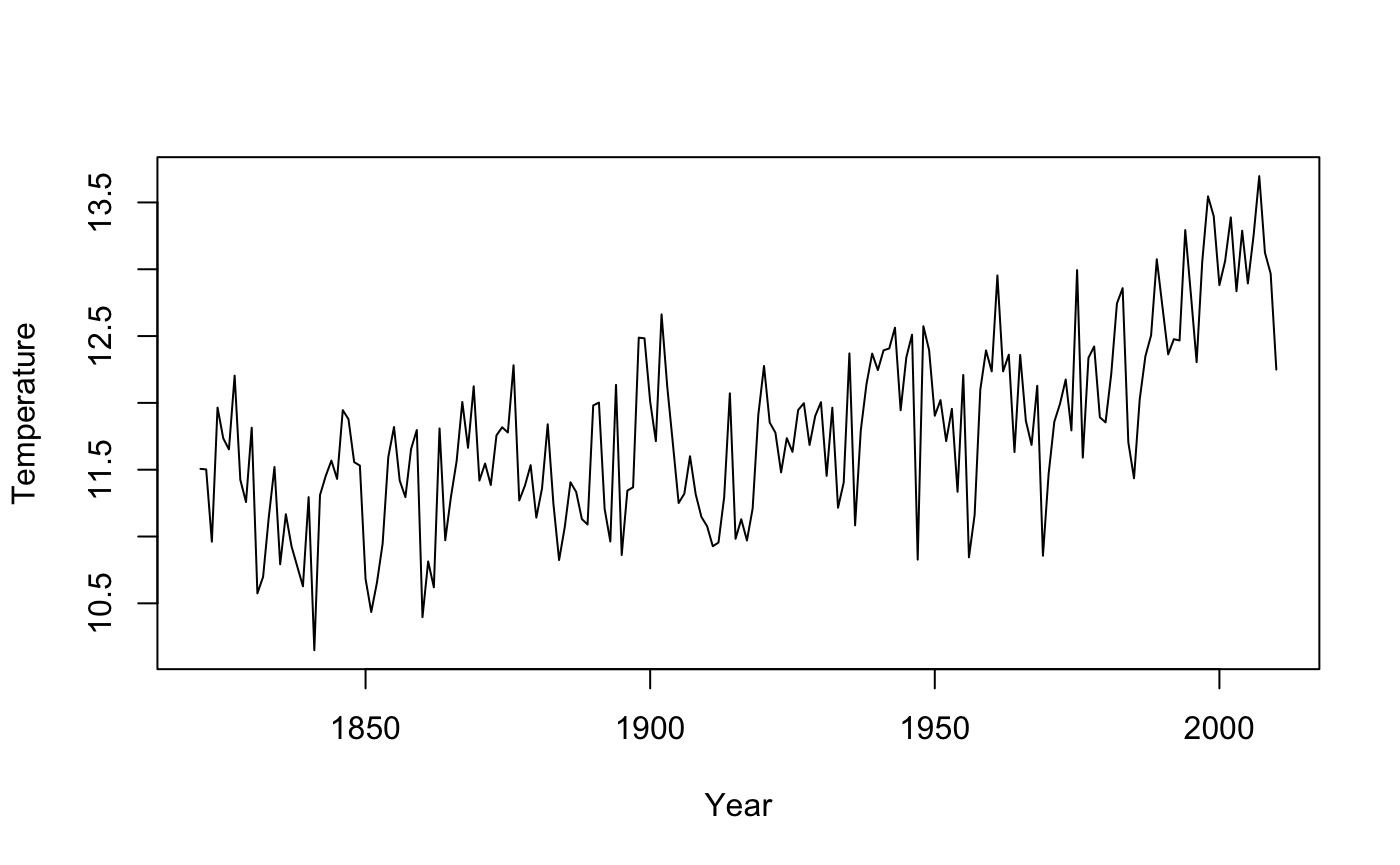
\includegraphics{/Users/mu/Desktop/Spring 2023/PSTAT 174/Final Project/original_data.png}\\

~~~~~~From the time series plot above, I noticed that there is an
increasing trend but no seasonal component. Also, I noticed the change
in trend. To be more specific, even though the overall trend of this
graph is increasing, we can see that the data increased very slowly
before 1950. However, the rate of increase goes up significantly after
1950. The potential reason that leads to this phenomenon is that the
People's Republic of China was established in 1949, and China has
started industrialization since then. Human activities, such as
industrialization, released large amounts of carbon dioxide, which
changed the earth's climate and increased the temperature.

\hypertarget{transformation-and-differencing}{%
\subsection{Transformation and
Differencing}\label{transformation-and-differencing}}

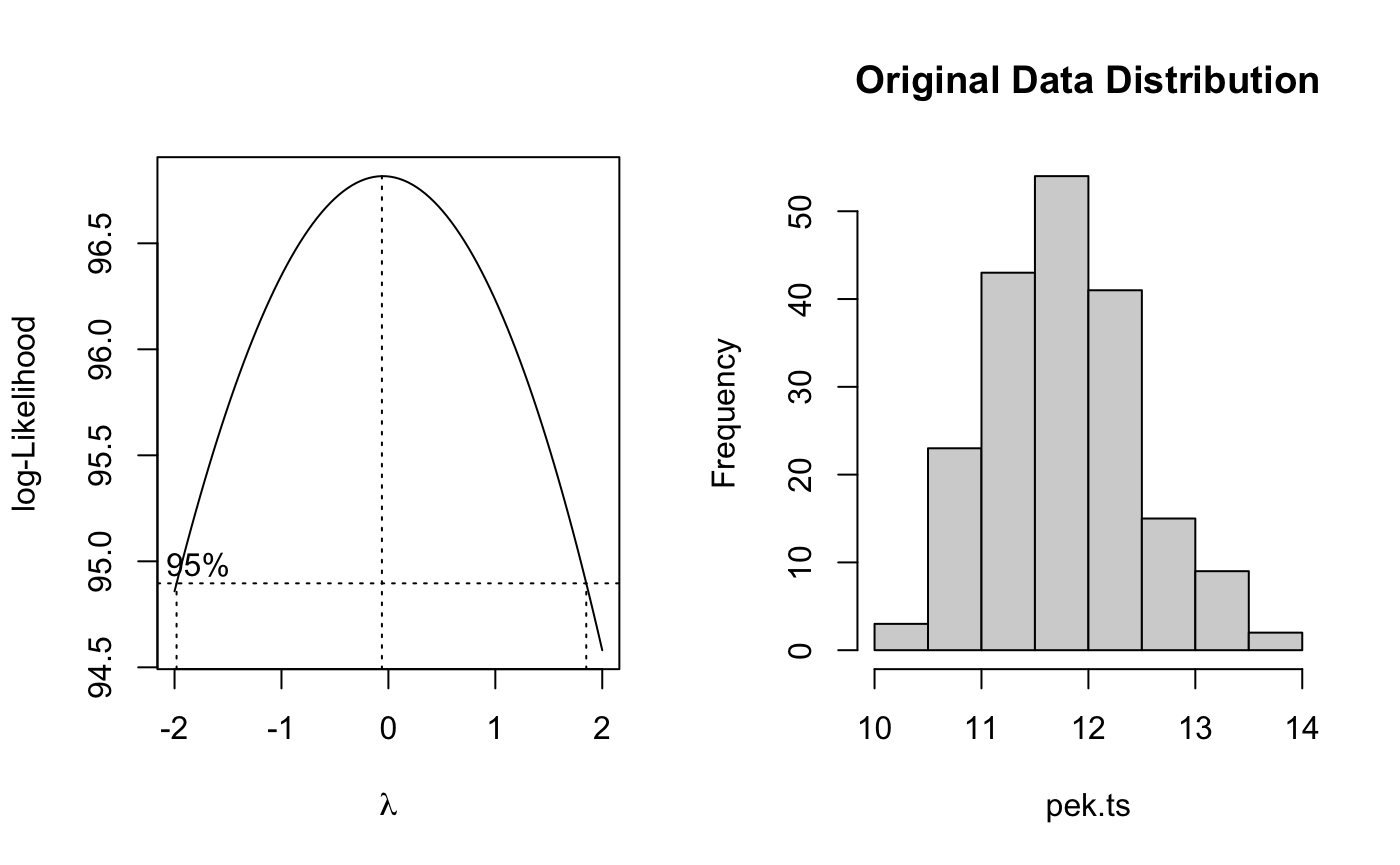
\includegraphics{/Users/mu/Desktop/Spring 2023/PSTAT 174/Final Project/transformation.png}\\

~~~~~~The plot on the left is the Box-Cox plot. It shows that 1 is
within the 95\% Confidence Interval for the value of \(\lambda\). Also,
the histogram on the right shows us the distribution of the original
data. It appears to be normally distributed and has a bell shape. Hence,
it's safe to conclude that a transformation is not necessary, and I
decided not to transform the data.

~~~~~~I differenced the data at lag one to eliminate the trend since I
observed an increasing trend. But I don't have to difference the data at
other lag since I didn't observe any seasonal component, and it's also
not reasonable to have seasonality in yearly data. After I differenced
the data once at lag 1, the variance decreased from 0.48 to 0.33.
However, after I differenced twice at lag 1, the variance increased to
0.93, which means over differencing. Hence, I decided to only difference
the data once at lag one.

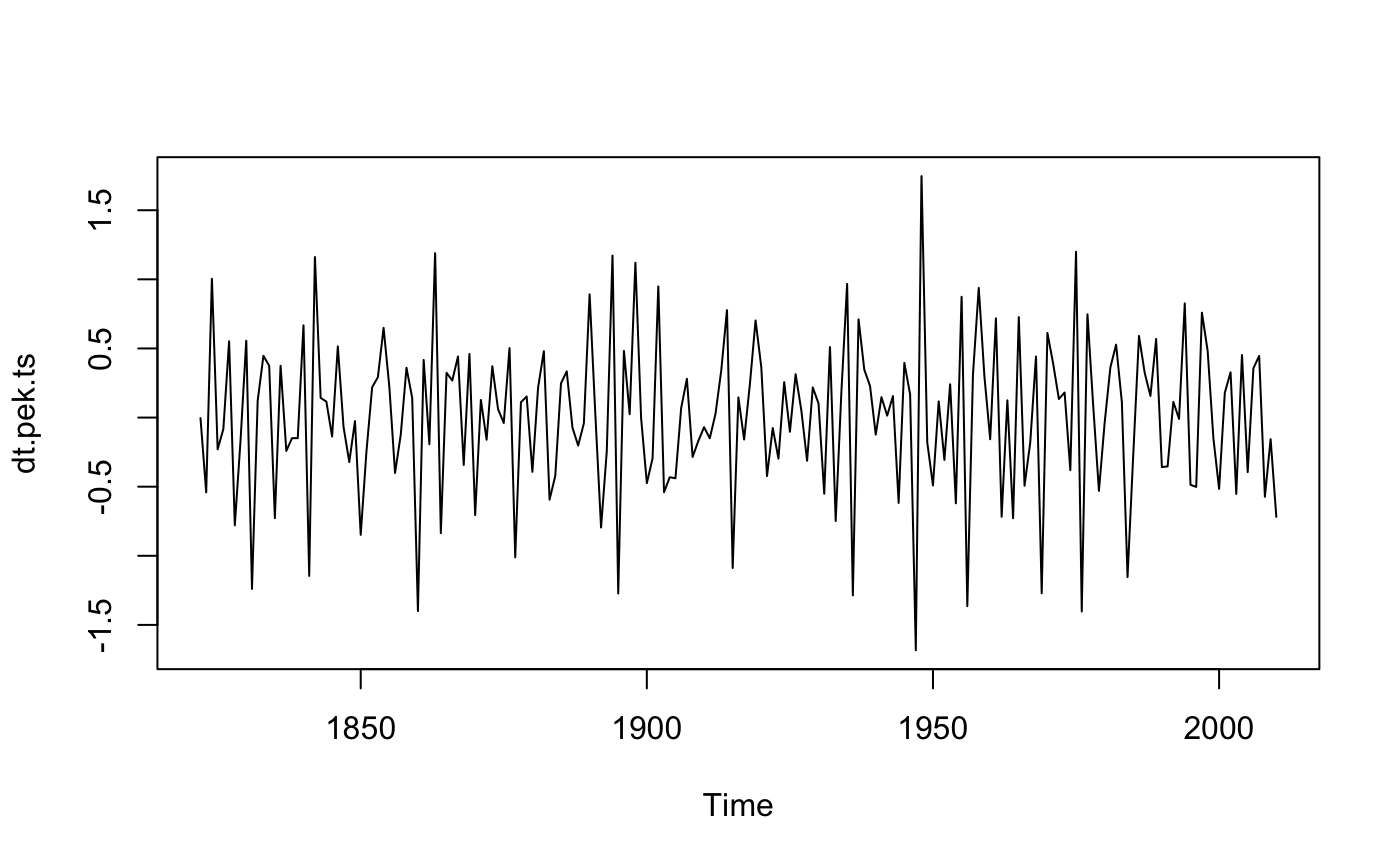
\includegraphics{/Users/mu/Desktop/Spring 2023/PSTAT 174/Final Project/detrend.png}\\

~~~~~~The plot above is the data after differencing once at lag one, or
the de-trended data. As we can see, there is no trend and the variance
looks stable over time, so it's safe to conclude that my time series
data is stationary now.

\hypertarget{preliminary-model-identification}{%
\subsection{Preliminary Model
Identification}\label{preliminary-model-identification}}

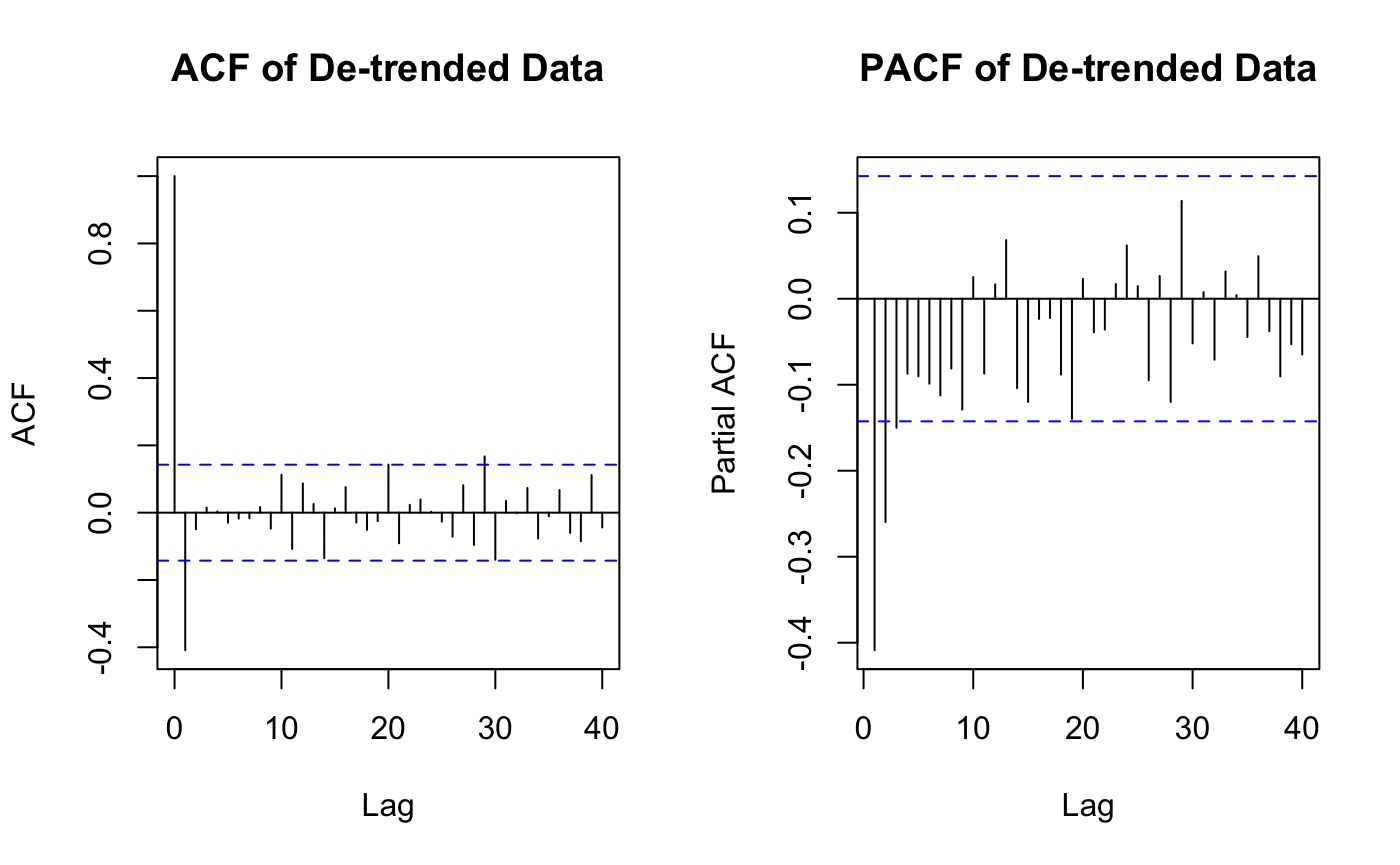
\includegraphics{/Users/mu/Desktop/Spring 2023/PSTAT 174/Final Project/acf_pacf.png}\\

~~~~~~The ACF plot shows that the ACF is statistically insignificant for
lag greater than 1, and the PACF plot shows that the PACF is
statistically insignificant for lag greater than 3. Also, we differenced
data once at lag one. So the potential values of the parameters in my
model are:

\begin{itemize}
\tightlist
\item
  p: 0,1,2,3
\item
  d: 1
\item
  q: 0,1
\end{itemize}

~~~~~~After knowing the potential values of the parameters, I run the
for loop to try different models and compared the model fits using AICc:

\begin{longtable}[]{@{}cccc@{}}
\toprule\noalign{}
& q & & \\
\midrule\noalign{}
\endhead
\bottomrule\noalign{}
\endlastfoot
p & & 0 & 1 \\
& 0 & 329.0586 & 270.5249 \\
& 1 & 296.4201 & 265.7672 \\
& 2 & 284.8366 & 265.8102 \\
& 3 & 281.9829 & 266.3851 \\
\end{longtable}

~~~~~~I chose 2 models with lowest AICc from the table above:
\(ARIMA(1,1,1)\) with AICc = 265.7672 and \(ARIMA(2,1,1)\) with AICc =
265.8102.

\hfill\break

\hypertarget{coefficients-estimation-and-diagnostic-checking}{%
\subsection{Coefficients Estimation and Diagnostic
Checking}\label{coefficients-estimation-and-diagnostic-checking}}

\hypertarget{coefficients-estimation}{%
\subsubsection{Coefficients Estimation}\label{coefficients-estimation}}

Let \textbf{\(X_t\)} denotes our original data,

\begin{itemize}
\tightlist
\item
  ARIMA(1,1,1):
  \((1-0.2373_{0.0963}B)\nabla_1X_t = (1-0.8656_{0.0547}B)Z_t\) with
  \(\hat{\sigma}^2_Z = 0.2308\)
\end{itemize}

\begin{longtable}[]{@{}ccc@{}}
\toprule\noalign{}
Coefficients & ar1 & ma1 \\
\midrule\noalign{}
\endhead
\bottomrule\noalign{}
\endlastfoot
value & 0.2373 & -0.8656 \\
s.e. & 0.0963 & 0.05471 \\
\end{longtable}

\begin{itemize}
\tightlist
\item
  ARIMA(2,1,1):
  \((1-0.2519_{0.0890}B - 0.0870_{0.0839}B^2)\nabla_1X_t = (1-0.8949_{0.0479}B)Z_t\)
  with \(\hat{\sigma}^2_Z = 0.2295\)
\end{itemize}

\begin{longtable}[]{@{}cccc@{}}
\toprule\noalign{}
Coefficients & ar1 & ar2 & ma1 \\
\midrule\noalign{}
\endhead
\bottomrule\noalign{}
\endlastfoot
value & 0.2519 & 0.0870 & -0.8949 \\
s.e. & 0.0890 & 0.0839 & 0.0479 \\
\end{longtable}

~~~~~~However, looking at the table, I noticed that the 95\% confidence
interval of \(\phi_2\), which is (-0.0808, 0.2548), contains zero.
Hence, it's better to set \(\phi_2 = 0\). But doing so will give us
\(ARIMA(1,1,1)\), which we already have. So I decided to go back to the
AICc matrix and find another model with low AICc.

\begin{longtable}[]{@{}cccc@{}}
\toprule\noalign{}
& q & & \\
\midrule\noalign{}
\endhead
\bottomrule\noalign{}
\endlastfoot
p & & 0 & 1 \\
& 0 & 329.0586 & 270.5249 \\
& 1 & 296.4201 & 265.7672 \\
& 2 & 284.8366 & 265.8102 \\
& 3 & 281.9829 & 266.3851 \\
\end{longtable}

~~~~~~From the table, I found out that \(ARIMA(3,1,1)\) and
\(ARIMA(0,1,1)\) also have very low AICc in comparison with other
models. So I decided to fit the data into \(ARIMA(0,1,1)\) with AICc =
270.5249 and \(ARIMA(3,1,1)\) with AICc = 266.3851.

\begin{itemize}
\tightlist
\item
  ARIMA(0,1,1): \(\nabla_1X_t = (1-0.7186_{0.0742}B)Z_t\) with
  \(\hat{\sigma}^2_Z = 0.2371\)
\end{itemize}

\begin{longtable}[]{@{}cc@{}}
\toprule\noalign{}
Coefficients & ma1 \\
\midrule\noalign{}
\endhead
\bottomrule\noalign{}
\endlastfoot
value & -0.7186 \\
s.e. & 0.0742 \\
\end{longtable}

\begin{itemize}
\tightlist
\item
  ARIMA(3,1,1):
  \((1-0.2641_{0.0865}B - 0.0851_{0.0818}B^2 - 0.0672_{0.0800}B^3)\nabla_1X_t = (1-0.9118_{0.0443}B)Z_t\)
  with \(\hat{\sigma}^2_Z = 0.2286\)
\end{itemize}

\begin{longtable}[]{@{}ccccc@{}}
\toprule\noalign{}
Coefficients & ar1 & ar2 & ar3 & ma1 \\
\midrule\noalign{}
\endhead
\bottomrule\noalign{}
\endlastfoot
value & 0.2641 & 0.0851 & 0.0672 & -0.9118 \\
s.e. & 0.0865 & 0.0818 & 0.0800 & 0.0443 \\
\end{longtable}

~~~~~~This \(ARIMA(3,1,1)\) has same issue as \(ARIMA(2,1,1)\). That is,
the 95\% confidence interval of \(\phi_2\), which is (-0.0785, 0.2487),
contains zero and the 95\% confidence interval of \(\phi_3\), which is
(-0.0928, 0.2272), contains zero as well. Hence, it's better to set
\(\phi_2 = \phi_3 = 0\). But doing so will give us \(ARIMA(1,1,1)\),
which we already have. Thus, I decided to only take \(ARIMA(1,1,1)\) and
\(ARIMA(0,1,1)\) to diagnostic checking.

\hypertarget{diagnostic-checking}{%
\subsubsection{Diagnostic Checking}\label{diagnostic-checking}}

\begin{itemize}
\tightlist
\item
  For \(ARIMA(1,1,1)\):
\end{itemize}

\((1-0.2373_{0.0963}B)\nabla_1X_t = (1-0.8656_{0.0547}B)Z_t\) with
\(\hat{\sigma}^2_Z = 0.2308\)

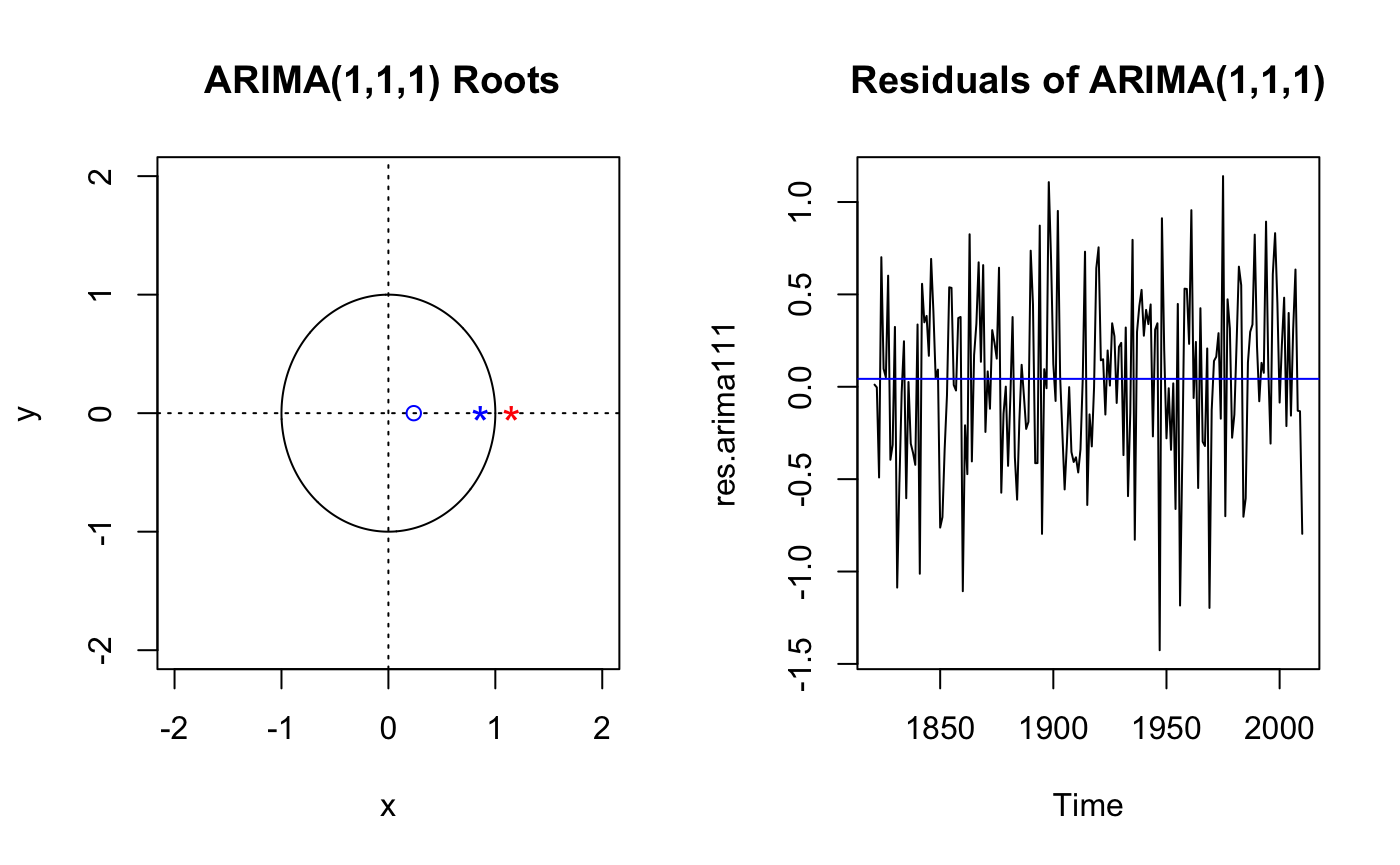
\includegraphics{/Users/mu/Desktop/Spring 2023/PSTAT 174/Final Project/a.1.png}\\

~~~~~~From the plots above, I found out that the roots of both Auto
Regressive characteristic polynomial and Moving Average characteristic
polynomial are outside of the unit circle. Also, I noticed that
\(|\theta_1| < 1\) and \(|\phi_1| < 1\), so it's safe to conclude that
this model is both stationary and invertible. The plot of the residuals
shows no trend, no visible change of variance, no seasonality, and the
sample mean is almost zero.

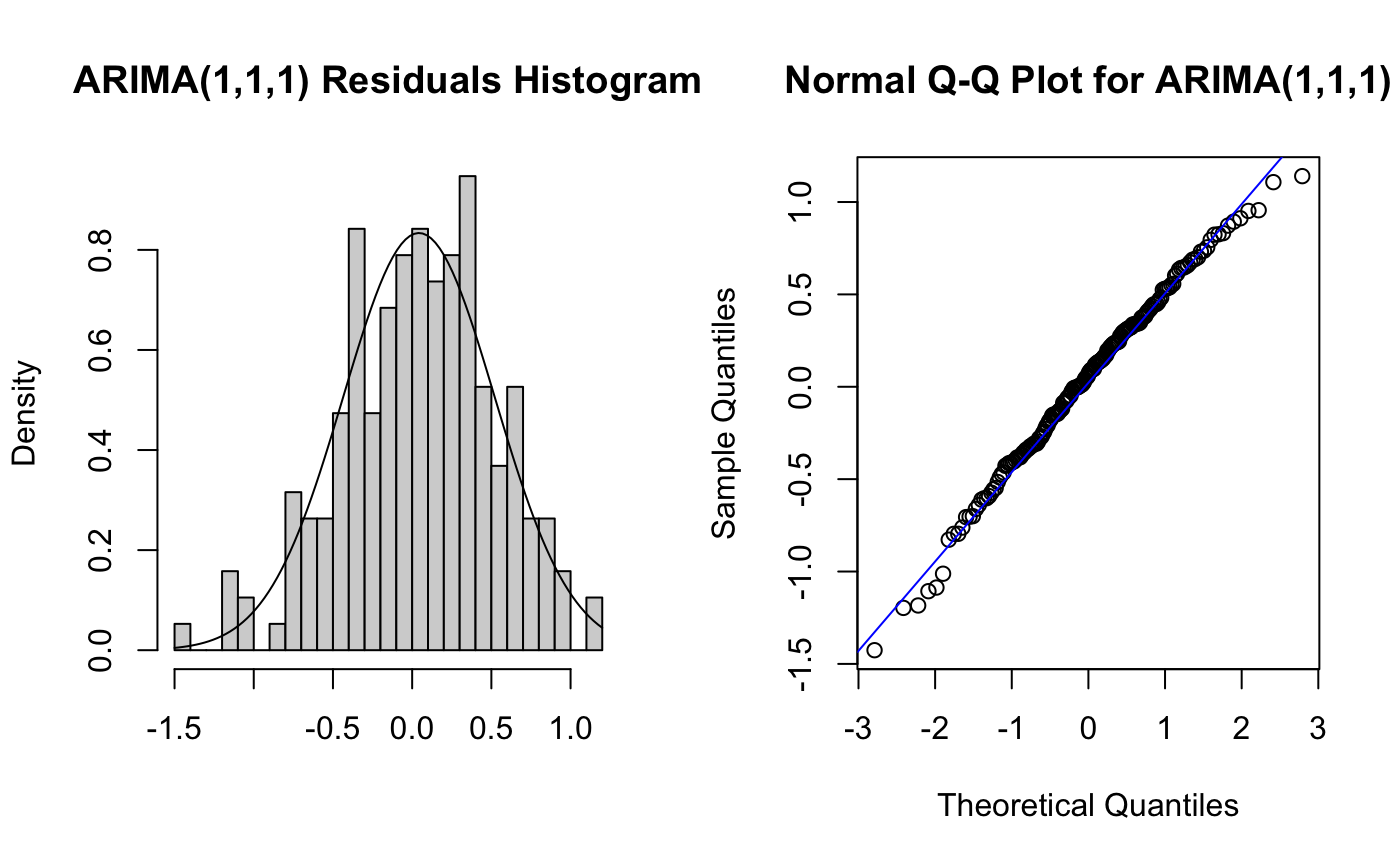
\includegraphics{/Users/mu/Desktop/Spring 2023/PSTAT 174/Final Project/a.2.png}\\

~~~~~~The histogram above indicates that the residuals appear to be
normally distributed since it has a bell shape. Moreover, in the Q-Q
plot, more than 95\% of the points are between -2 and 2, which again
indicates the residuals follow normal distribution.

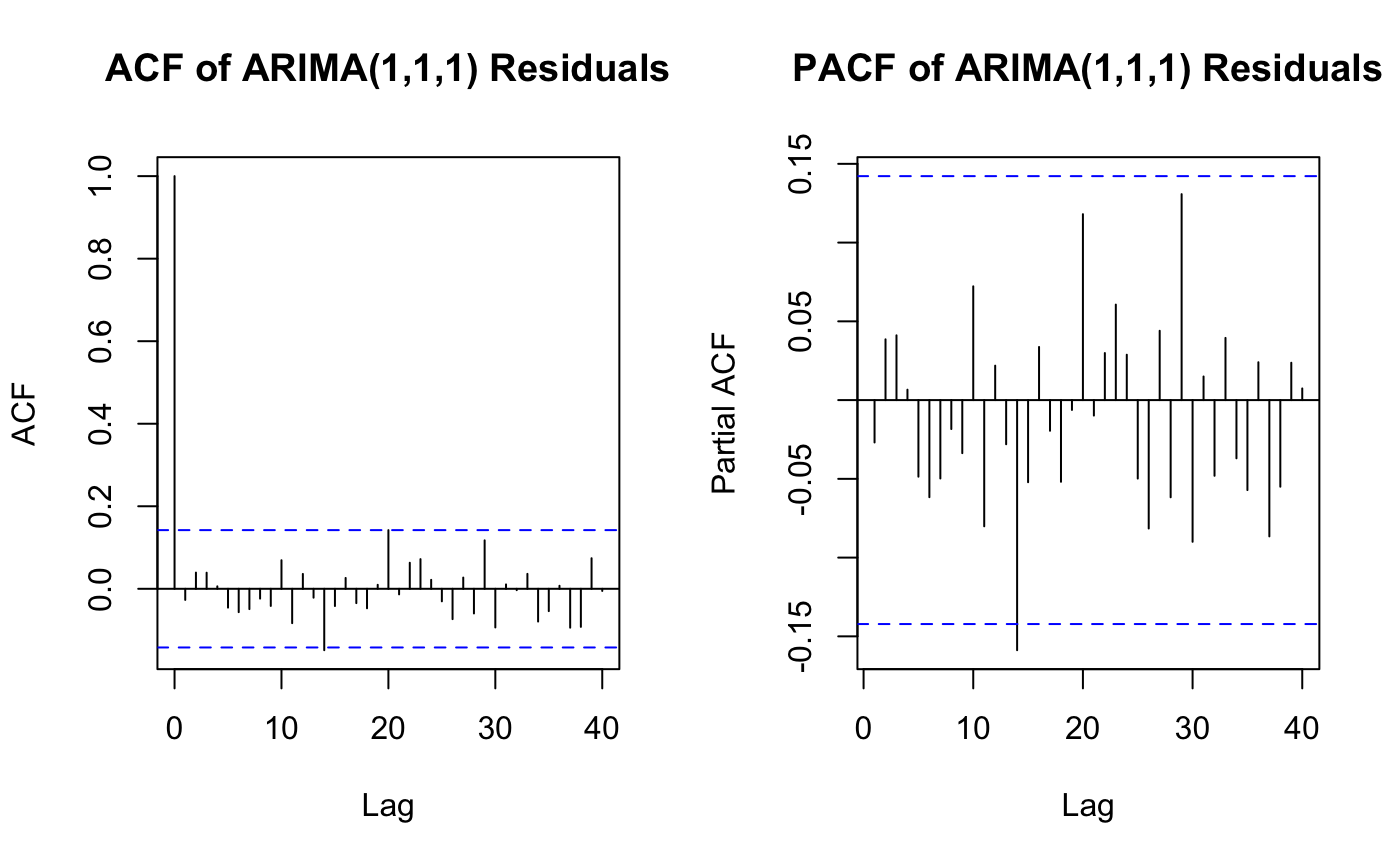
\includegraphics{/Users/mu/Desktop/Spring 2023/PSTAT 174/Final Project/a.3.png}\\

~~~~~~From the plots above, I found out that all the ACF of residuals
are within the confidence interval, which can be counted as zeros.
However, I noticed that PACF at lag 14 is slightly out of the confidence
interval, and I decided to see the results of other tests. It doesn't
matter if the residuals of this model pass all other tests.

\hfill\break

\begin{longtable}[]{@{}cc@{}}
\toprule\noalign{}
Tests & P-value/ Test Result \\
\midrule\noalign{}
\endhead
\bottomrule\noalign{}
\endlastfoot
Shapiro-Wilk Normality Test & 0.4014 \\
Box-Pierce Test & 0.6692 \\
Ljung-Box Test & 0.6104 \\
Mcleod-Li Test & 0.3185 \\
AR Order Select & 0 \\
\end{longtable}

~~~~~~The table above shows the P-value of the Shapiro-Wilk normality
test, Box-Pierce test, Ljung-Box test, and Mcleod-Li test. This model
passed all these tests since the P-values were all larger than 0.05.
Moreover, I plugged the residuals from this model into the Yule-Walker
method, and it automatically selected 0, which means white noise. Since
the residuals of the \(ARIMA(1,1,1)\) model passed all the tests, it's
safe to say that PACF at lag 14 slightly out of the confidence interval
doesn't matter and we can move on to the next model.

\begin{itemize}
\tightlist
\item
  For \(ARIMA(0,1,1)\):
\end{itemize}

\(\nabla_1X_t = (1-0.7186_{0.0742}B)Z_t\) with
\(\hat{\sigma}^2_Z = 0.2371\)

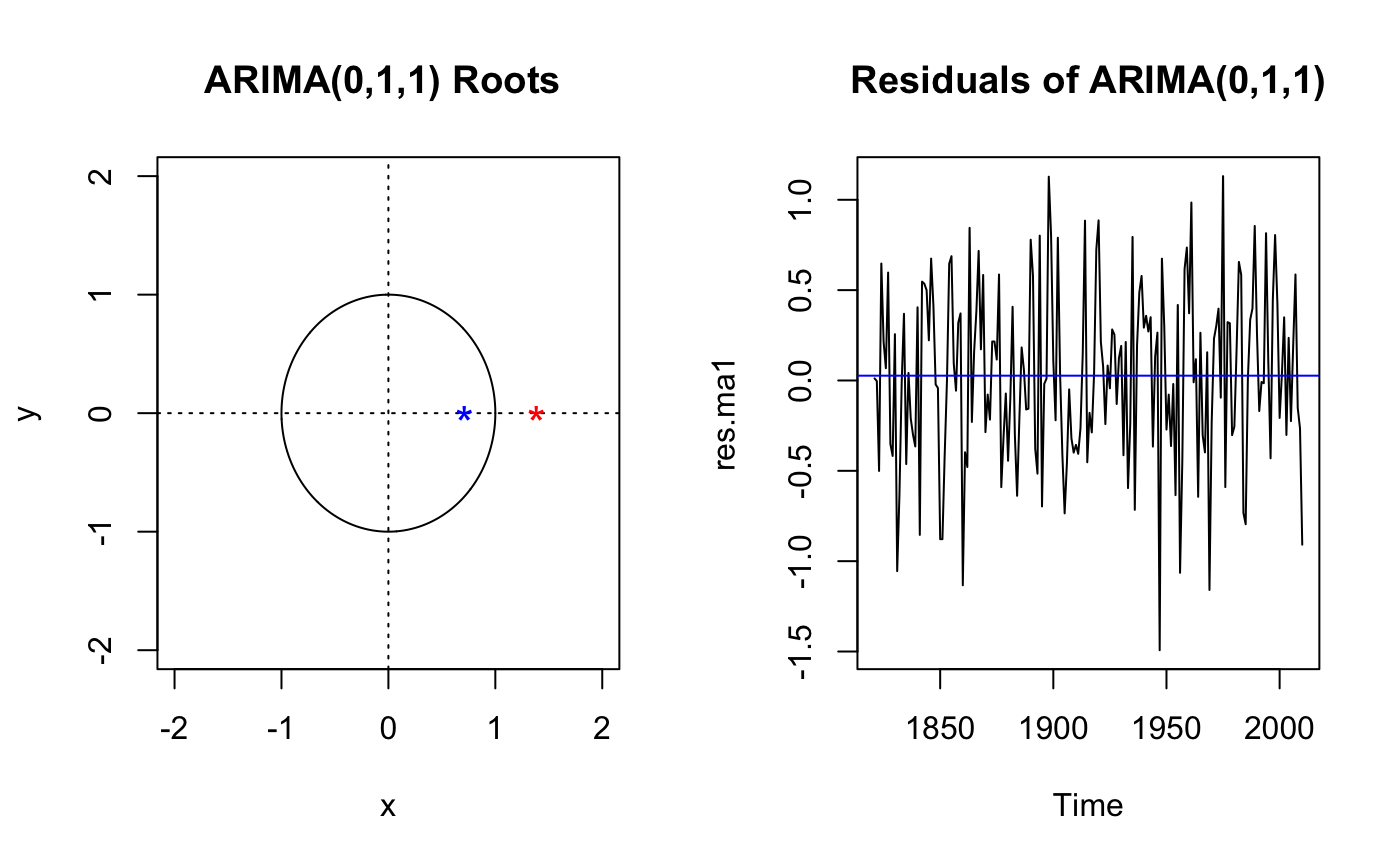
\includegraphics{/Users/mu/Desktop/Spring 2023/PSTAT 174/Final Project/b.1.png}\\

~~~~~~From the plots above, I found out that the root of the
characteristic polynomial are outside of the unit circle. Also, I
noticed that \(|\theta_1| < 1\), so it's safe to conclude that this
model is both stationary and invertible. The plot of the residuals shows
no trend, no visible change of variance, no seasonality, and the sample
mean is almost zero.

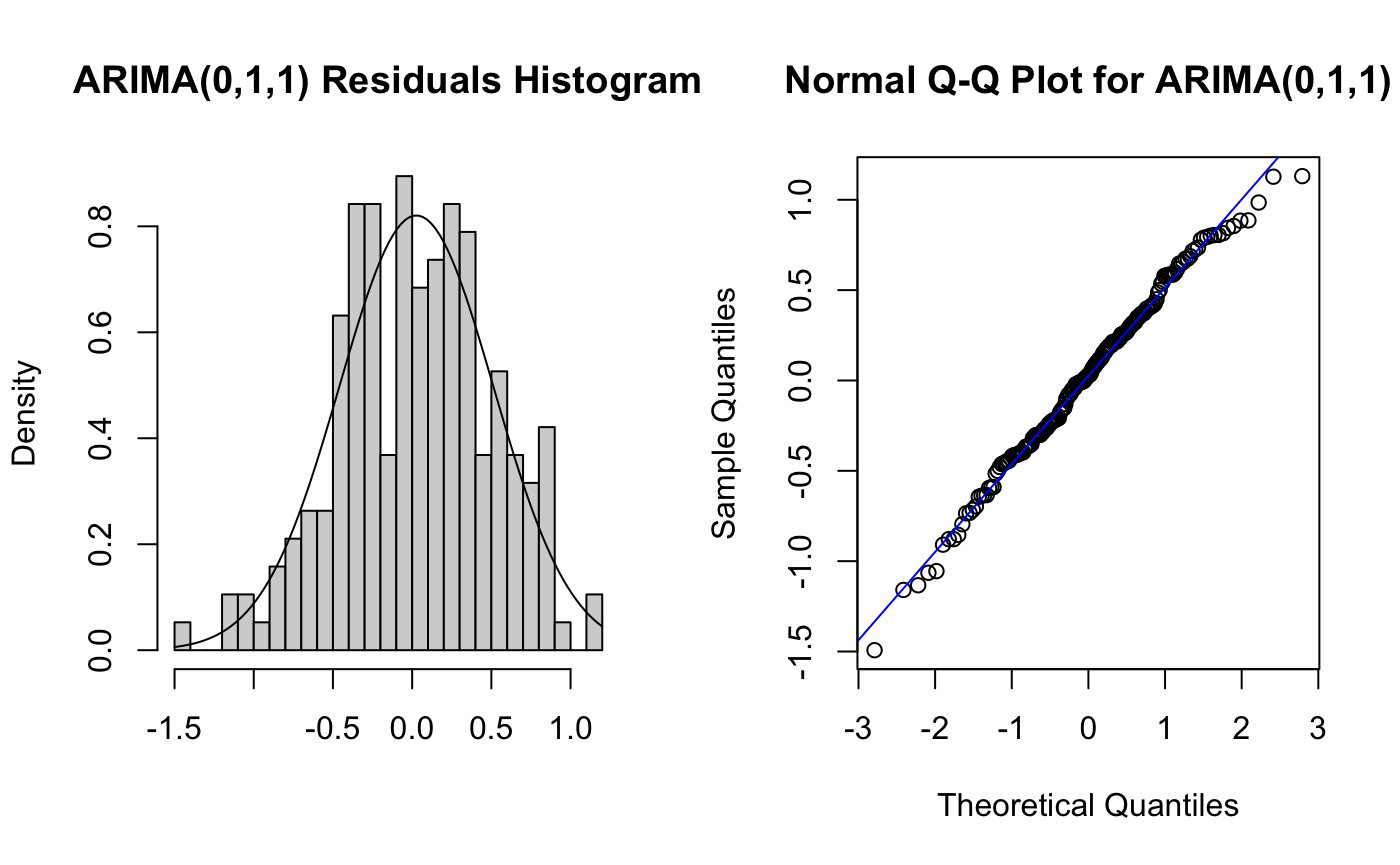
\includegraphics{/Users/mu/Desktop/Spring 2023/PSTAT 174/Final Project/b.2.png}\\

~~~~~~The histogram above indicates that the residuals appear to be
normally distributed since it has a bell shape. Moreover, in the Q-Q
plot, more than 95\% of the points are between -2 and 2, which again
indicates the residuals follow normal distribution.

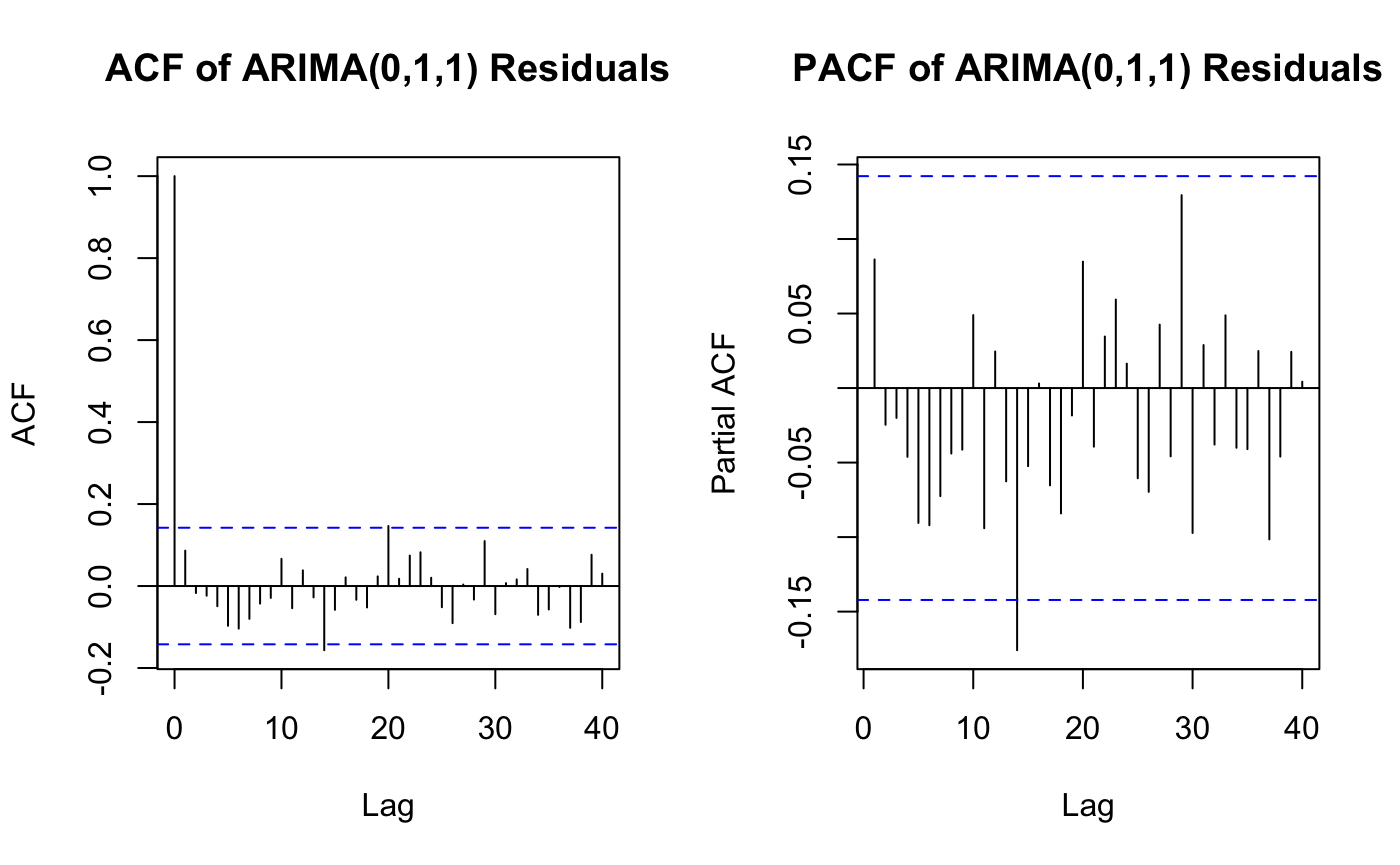
\includegraphics{/Users/mu/Desktop/Spring 2023/PSTAT 174/Final Project/b.3.png}\\

~~~~~~From the plots above, I found out that all the ACF of residuals
are within the confidence interval, which can be counted as zeros.
However, I noticed that PACF at lag 14 is slightly out of the confidence
interval, and I decided to see the results of other tests. It doesn't
matter if the residuals of this model pass all other tests.

\hfill\break

\begin{longtable}[]{@{}cc@{}}
\toprule\noalign{}
Tests & P-value/ Test Result \\
\midrule\noalign{}
\endhead
\bottomrule\noalign{}
\endlastfoot
Shapiro-Wilk Normality Test & 0.4891 \\
Box-Pierce Test & 0.3696 \\
Ljung-Box Test & 0.3136 \\
Mcleod-Li Test & 0.4206 \\
AR Order Select & 0 \\
\end{longtable}

~~~~~~The table above shows the P-value of the Shapiro-Wilk normality
test, Box-Pierce test, Ljung-Box test, and Mcleod-Li test. This model
passed all these tests since the P-values were all larger than 0.05.
Moreover, I plugged the residuals from this model into the Yule-Walker
method, and it automatically selected 0, which means white noise. Since
the residuals of the \(ARIMA(0,1,1)\) model passed all the tests, it's
safe to say that PACF at lag 14 slightly out of the confidence interval
doesn't matter.

\begin{itemize}
\tightlist
\item
  Final Model Selection:
\end{itemize}

~~~~~~As we can see, both models passed all the tests. According to the
principle of parsimony, I should choose the one with the least
coefficients, which is the \(ARIMA(0,1,1)\) model.This final model
obtained by using AICc and the principle of parsimony is one of the
models suggested by ACF and PACF. Since my final model passed all the
tests on residuals of the model, I can conclude that my final model is
satisfactory. Finally, my final model in algebraic form is:
\(\nabla_1X_t = (1-0.7186_{0.0742}B)Z_t\) with
\(\hat{\sigma}^2_Z = 0.2371\).

\hypertarget{forecasting}{%
\subsection{Forecasting}\label{forecasting}}

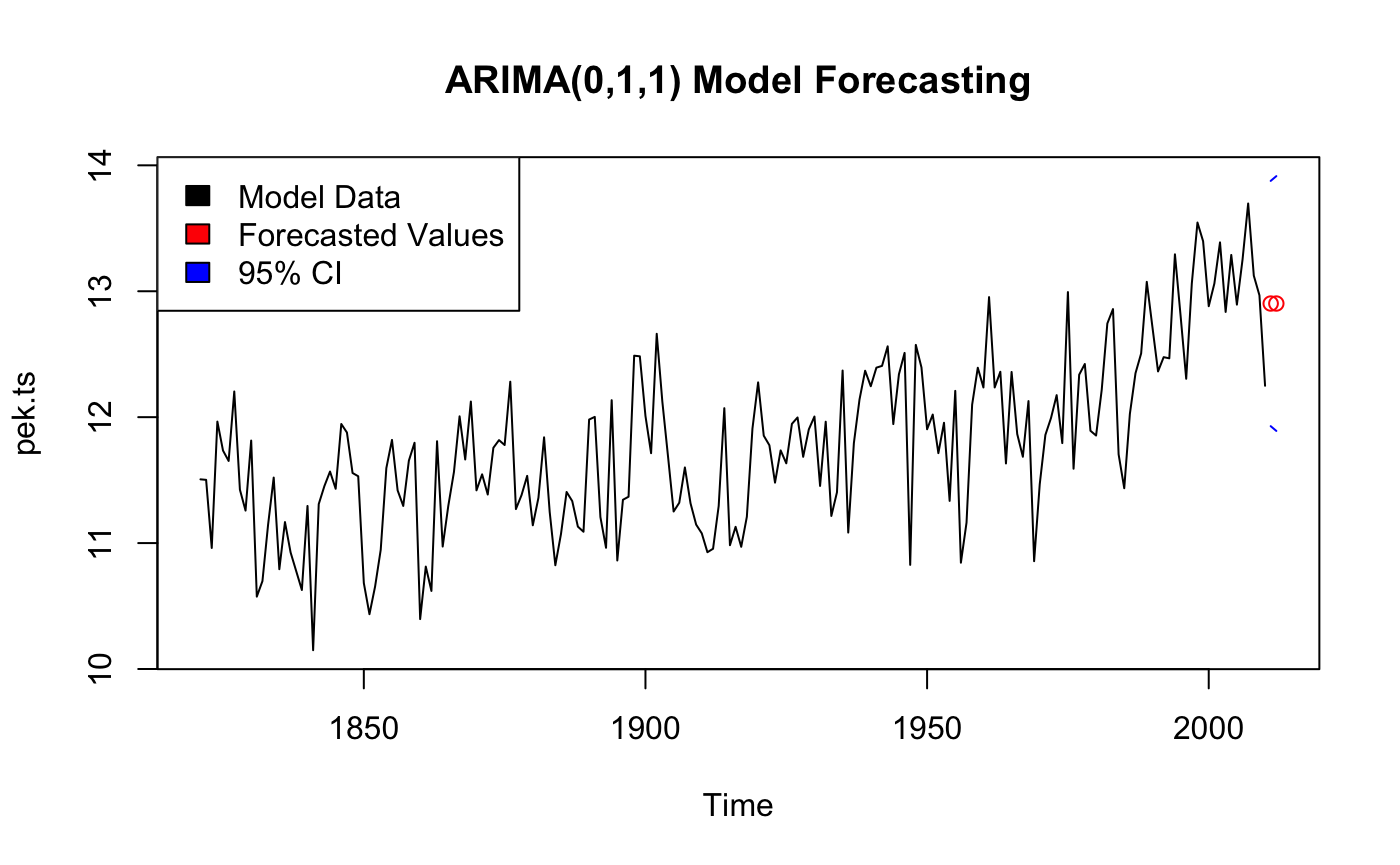
\includegraphics{/Users/mu/Desktop/Spring 2023/PSTAT 174/Final Project/f1.png}
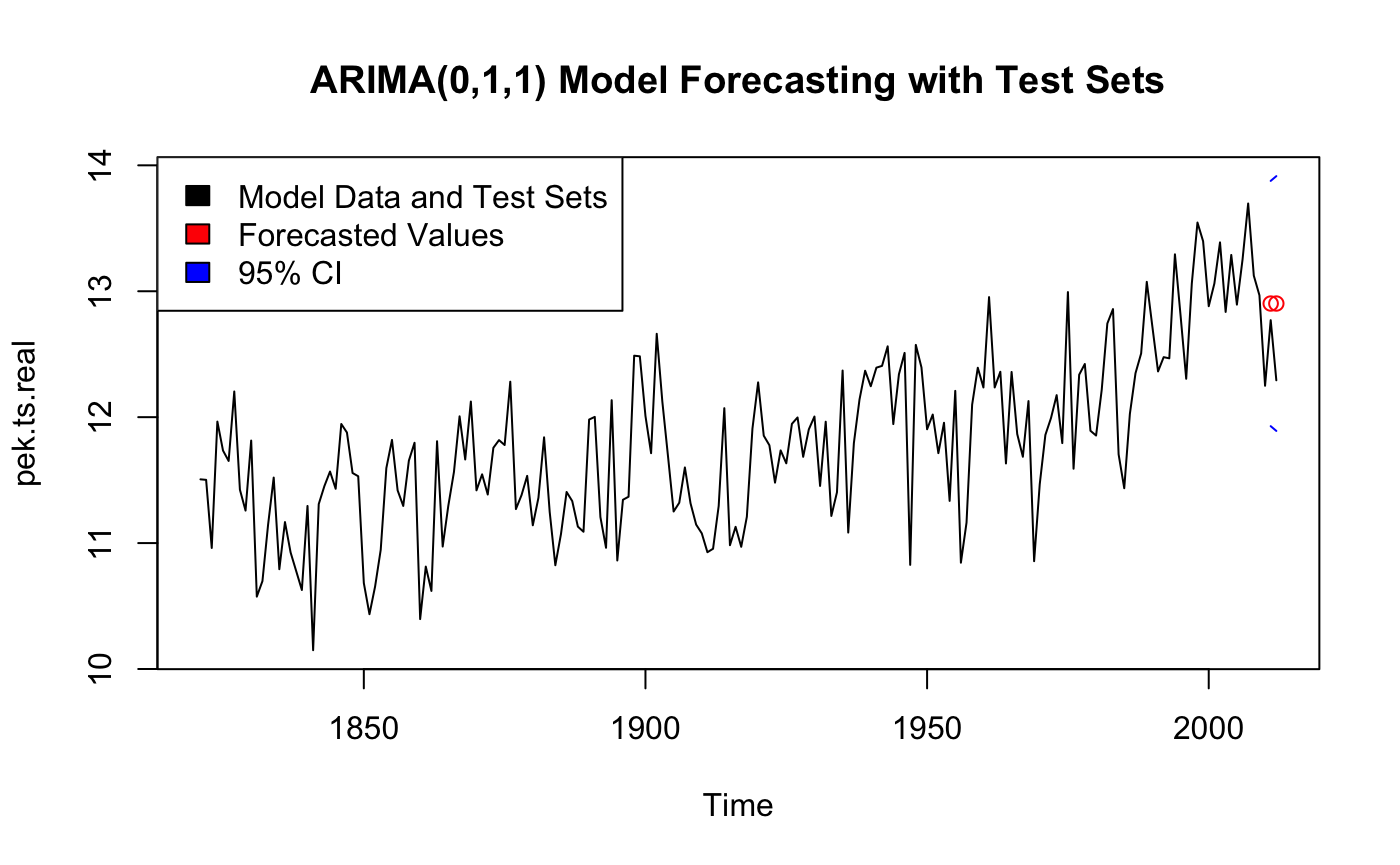
\includegraphics{/Users/mu/Desktop/Spring 2023/PSTAT 174/Final Project/f2.png}
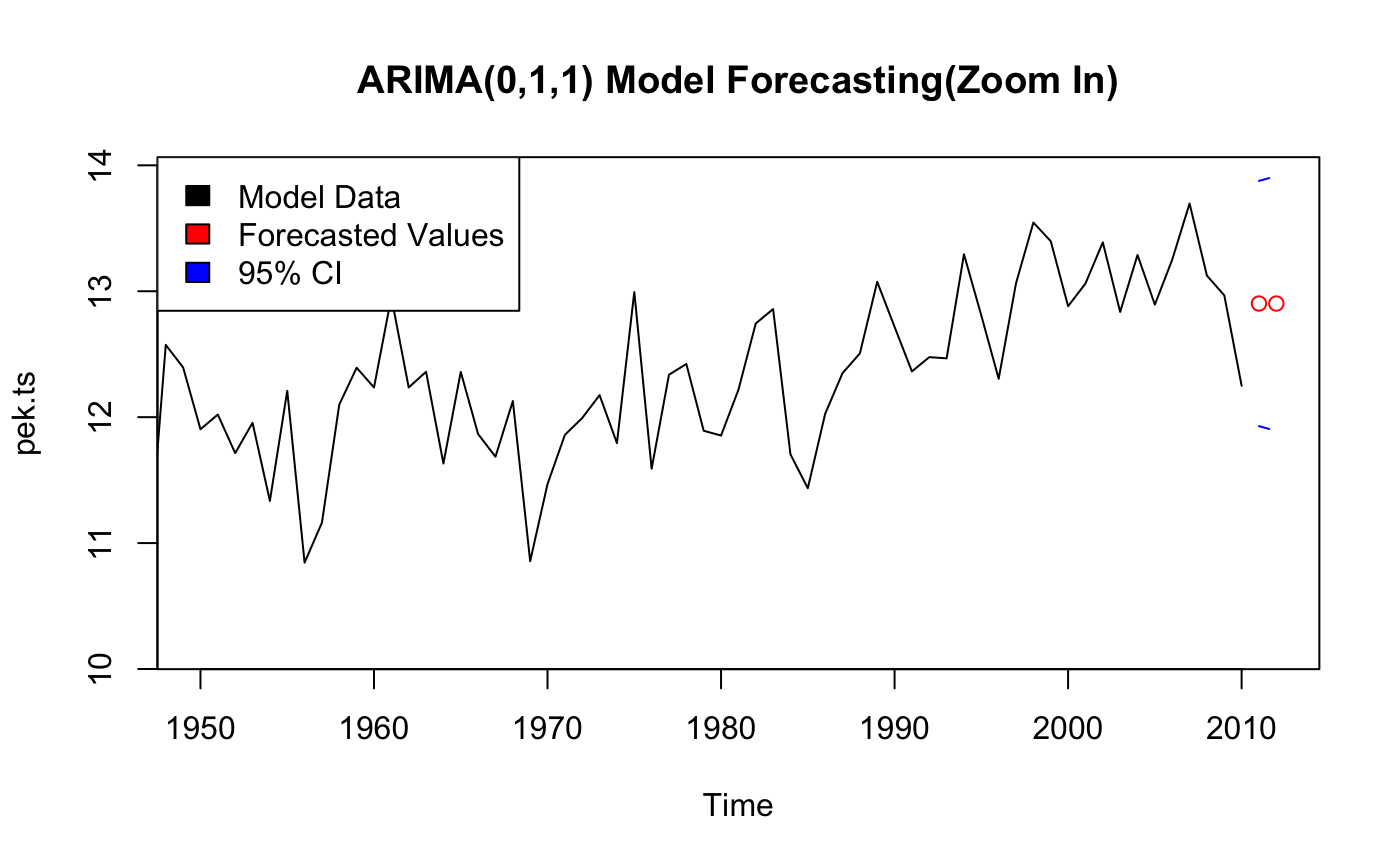
\includegraphics{/Users/mu/Desktop/Spring 2023/PSTAT 174/Final Project/fz1.png}
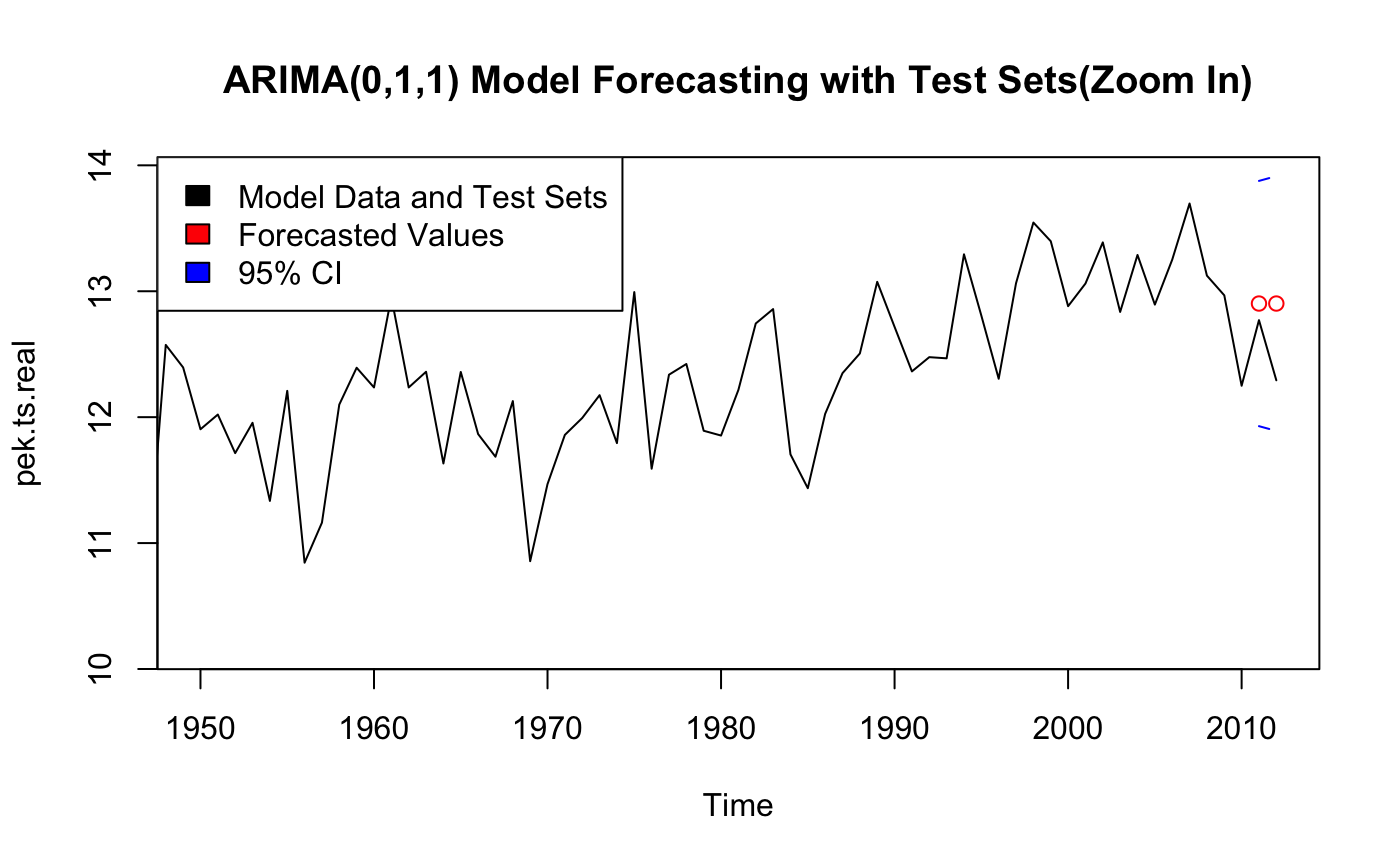
\includegraphics{/Users/mu/Desktop/Spring 2023/PSTAT 174/Final Project/fz2.png}\\

~~~~~~The first two plots include the original series, forecasted values
using my final model, and the confidence interval for the forecasted
values. I also included two zoom-in plots of the first two plots to be
able to see the detail clearly. From the plots, I noticed that the test
sets are within the confidence intervals, which means this model is
satisfactory and I have successfully addressed my problem.

\hypertarget{conclusion}{%
\subsection{Conclusion}\label{conclusion}}

~~~~~~In conclusion, I successfully achieved my goal of training a model
to forecast the yearly temperature of Peking. The math formula for my
final model is \(\nabla_1X_t = (1-0.7186_{0.0742}B)Z_t\). I used the
final model for forecasting, and the test sets are within the prediction
intervals, which again confirmed that my model is satisfactory. Hence, I
successfully achieved my goal.

~~~~~~Professor Feldman strongly supported me in this final project. Her
lectures and slides built me a solid foundation in time series
knowledge. More importantly, when I encountered detailed problems, I
could always schedule office hour appointments with her and discuss the
problems.

\hypertarget{references}{%
\subsection{References}\label{references}}

\hypertarget{refs}{}
\begin{CSLReferences}{1}{0}
\leavevmode\vadjust pre{\hypertarget{ref-Data}{}}%
Berkeley, Earth. 1 May, 2017. \emph{{``Climate Change: Earth Surface
Temperature Data.''}} Kaggle.
\href{https://www.kaggle.com/datasets/berkeleyearth/climate-change-earth-surface-temperature-data}{www.kaggle.com/datasets/berkeleyearth/climate-change-earth-surface-temperature-data}.

\leavevmode\vadjust pre{\hypertarget{ref-Slides15}{}}%
Feldman, Raisa. 2023. \emph{Lecture 15 Slides-Example of a Project}.

\end{CSLReferences}

\hypertarget{appendix}{%
\subsection{Appendix}\label{appendix}}

\begin{Shaded}
\begin{Highlighting}[]
\CommentTok{\# Data Tidying}
\NormalTok{raw }\OtherTok{\textless{}{-}} \FunctionTok{read.csv}\NormalTok{(}\StringTok{\textquotesingle{}GlobalLandTemperaturesByMajorCity.csv\textquotesingle{}}\NormalTok{) }\CommentTok{\# Read in the data}
\NormalTok{pek.temp }\OtherTok{\textless{}{-}}\NormalTok{ raw[raw}\SpecialCharTok{$}\NormalTok{City }\SpecialCharTok{==} \StringTok{"Peking"}\NormalTok{, }\DecValTok{1}\SpecialCharTok{:}\DecValTok{2}\NormalTok{] }\CommentTok{\# Filter observations on Peking(Date\&Temperature)}
\NormalTok{pek.temp }\OtherTok{\textless{}{-}}\NormalTok{ pek[,}\DecValTok{1}\SpecialCharTok{:}\DecValTok{2}\NormalTok{] }\CommentTok{\# Filter variables: only date and average temperature}
\FunctionTok{sum}\NormalTok{(}\FunctionTok{is.na}\NormalTok{(pek.temp)) }\CommentTok{\# Total number of missing values}
\NormalTok{pek.temp[}\FunctionTok{is.na}\NormalTok{(pek.temp}\SpecialCharTok{$}\NormalTok{AverageTemperature) }\SpecialCharTok{==} \ConstantTok{TRUE}\NormalTok{,] }\CommentTok{\# Distribution of missing values}
\NormalTok{pek.temp[}\StringTok{"176394"}\NormalTok{,}\StringTok{"AverageTemperature"}\NormalTok{] }\OtherTok{\textless{}{-}}\NormalTok{ (pek.temp[}\StringTok{"176395"}\NormalTok{,}\StringTok{"AverageTemperature"}\NormalTok{]}\SpecialCharTok{+}
\NormalTok{                                              pek.temp[}\StringTok{"176393"}\NormalTok{,}\StringTok{"AverageTemperature"}\NormalTok{]) }\SpecialCharTok{/}\DecValTok{2} 
\CommentTok{\# October 1832: mean of neighbor months\textquotesingle{} average temperature}
\NormalTok{pek.temp[}\StringTok{"178565"}\NormalTok{,}\StringTok{"AverageTemperature"}\NormalTok{] }\OtherTok{\textless{}{-}}\NormalTok{ (pek.temp[}\StringTok{"178563"}\NormalTok{,}\StringTok{"AverageTemperature"}\NormalTok{]}\SpecialCharTok{+}
\NormalTok{                                              pek.temp[}\StringTok{"178564"}\NormalTok{,}\StringTok{"AverageTemperature"}\NormalTok{])}\SpecialCharTok{/}\DecValTok{2} 
\CommentTok{\#September 2013: mean of previous two months\textquotesingle{} average temperature}
\ControlFlowTok{for}\NormalTok{ (index }\ControlFlowTok{in} \FunctionTok{as.character}\NormalTok{(}\FunctionTok{seq}\NormalTok{(}\DecValTok{176457}\NormalTok{,}\DecValTok{176468}\NormalTok{))) \{}
\NormalTok{  pek.temp[index, }\StringTok{"AverageTemperature"}\NormalTok{] }\OtherTok{\textless{}{-}} \DecValTok{0}
\NormalTok{\} }\CommentTok{\# 1838 all year fill 0 first}
\FunctionTok{sum}\NormalTok{(}\FunctionTok{is.na}\NormalTok{(pek.temp)) }\CommentTok{\# Check missing values after the operations above}
\NormalTok{pek.temp }\OtherTok{\textless{}{-}}\NormalTok{ pek.temp[}\FunctionTok{as.character}\NormalTok{(}\FunctionTok{seq}\NormalTok{(}\DecValTok{176253}\NormalTok{,}\DecValTok{178556}\NormalTok{)),] }
\CommentTok{\# Remove 1820 and 2013 since missing part of the year}
\NormalTok{year.temp }\OtherTok{\textless{}{-}} \FunctionTok{c}\NormalTok{()}
\ControlFlowTok{for}\NormalTok{ (jan }\ControlFlowTok{in} \FunctionTok{seq}\NormalTok{(}\DecValTok{1}\NormalTok{,}\DecValTok{2304}\NormalTok{,}\DecValTok{12}\NormalTok{))\{}
\NormalTok{  dec }\OtherTok{\textless{}{-}}\NormalTok{ jan}\SpecialCharTok{+}\DecValTok{11}
\NormalTok{  year.temp }\OtherTok{\textless{}{-}} \FunctionTok{c}\NormalTok{(year.temp,}\FunctionTok{mean}\NormalTok{(pek.temp[jan}\SpecialCharTok{:}\NormalTok{dec,}\DecValTok{2}\NormalTok{]))}
\NormalTok{\} }\CommentTok{\# Convert monthly data to yearly data by take the mean of 12 months}
\NormalTok{Year }\OtherTok{\textless{}{-}} \FunctionTok{c}\NormalTok{(}\DecValTok{1821}\SpecialCharTok{:}\DecValTok{2012}\NormalTok{) }\CommentTok{\# Year list}
\NormalTok{data }\OtherTok{\textless{}{-}} \FunctionTok{data.frame}\NormalTok{(}\AttributeTok{Year =}\NormalTok{ Year,}
                   \AttributeTok{AverageTemperature =}\NormalTok{ year.temp) }\CommentTok{\# Construct a data frame of tidied yearly data}
\NormalTok{data[data}\SpecialCharTok{$}\NormalTok{Year }\SpecialCharTok{==} \DecValTok{1838}\NormalTok{, }\StringTok{"AverageTemperature"}\NormalTok{] }\OtherTok{\textless{}{-}}\NormalTok{ (data[data}\SpecialCharTok{$}\NormalTok{Year }\SpecialCharTok{==} \DecValTok{1837}\NormalTok{, }\StringTok{"AverageTemperature"}\NormalTok{] }\SpecialCharTok{+} 
\NormalTok{                                                  data[data}\SpecialCharTok{$}\NormalTok{Year }\SpecialCharTok{==}\DecValTok{1839}\NormalTok{,}\StringTok{"AverageTemperature"}\NormalTok{])}\SpecialCharTok{/}\DecValTok{2}
\CommentTok{\# Initially, we set 1838 all year to be 0 for convenience. }
\CommentTok{\# Now, after we got yearly data, we fill the value of 1838 by the mean of neighbor years}
\NormalTok{model.data }\OtherTok{\textless{}{-}}\NormalTok{ data[Year }\SpecialCharTok{\textless{}=} \DecValTok{2010}\NormalTok{, ] }\CommentTok{\# Model data set: 190 observations}
\NormalTok{test.data }\OtherTok{\textless{}{-}}\NormalTok{ data[Year }\SpecialCharTok{\textgreater{}} \DecValTok{2010}\NormalTok{, ] }\CommentTok{\# Test set: 2 observations}

\CommentTok{\# Plot and Analyze}
\NormalTok{pek.ts }\OtherTok{\textless{}{-}} \FunctionTok{ts}\NormalTok{(model.data[,}\DecValTok{2}\NormalTok{], }\AttributeTok{start =} \DecValTok{1821}\NormalTok{, }\AttributeTok{frequency =} \DecValTok{1}\NormalTok{) }\CommentTok{\# Transform to time series object}
\FunctionTok{ts.plot}\NormalTok{(pek.ts, }\AttributeTok{gpars=}\FunctionTok{list}\NormalTok{(}\AttributeTok{xlab=}\StringTok{"Year"}\NormalTok{, }\AttributeTok{ylab=}\StringTok{"Temperature"}\NormalTok{)) }\CommentTok{\# Plot the time series}

\CommentTok{\# Transformation and Differencing}
\NormalTok{op }\OtherTok{\textless{}{-}} \FunctionTok{par}\NormalTok{(}\AttributeTok{mfrow=}\FunctionTok{c}\NormalTok{(}\DecValTok{1}\NormalTok{,}\DecValTok{2}\NormalTok{)) }\CommentTok{\# Box{-}Cox and Histogram to see if transformation is necessary}
\FunctionTok{library}\NormalTok{(MASS)}
\NormalTok{t }\OtherTok{=} \DecValTok{1}\SpecialCharTok{:}\FunctionTok{length}\NormalTok{(pek.ts)}
\NormalTok{fit }\OtherTok{=} \FunctionTok{lm}\NormalTok{(pek.ts }\SpecialCharTok{\textasciitilde{}}\NormalTok{ t)}
\NormalTok{bcTransform }\OtherTok{=} \FunctionTok{boxcox}\NormalTok{(pek.ts }\SpecialCharTok{\textasciitilde{}}\NormalTok{ t,}\AttributeTok{plotit =}\NormalTok{ T) }\CommentTok{\# See what lambda value boxcox gives us}
\FunctionTok{hist}\NormalTok{(pek.ts, }\AttributeTok{main =} \StringTok{\textquotesingle{}Original Data Distribution\textquotesingle{}}\NormalTok{)}\CommentTok{\# Check the distribution of original data}
\FunctionTok{par}\NormalTok{(op)}

\FunctionTok{var}\NormalTok{(pek.ts) }\CommentTok{\# Variance before Diff}
\NormalTok{dt.pek.ts }\OtherTok{\textless{}{-}} \FunctionTok{diff}\NormalTok{(pek.ts, }\DecValTok{1}\NormalTok{)}
\NormalTok{(}\FunctionTok{var}\NormalTok{(dt.pek.ts)) }\CommentTok{\# Variance after diff once at lag 1}
\NormalTok{dt2.pek.ts }\OtherTok{\textless{}{-}} \FunctionTok{diff}\NormalTok{(dt.pek.ts, }\DecValTok{1}\NormalTok{)}
\NormalTok{(}\FunctionTok{var}\NormalTok{(dt2.pek.ts)) }\CommentTok{\# Variance after diff twice at lag 1}
\FunctionTok{plot}\NormalTok{(dt.pek.ts) }\CommentTok{\# Plot of the de{-}trended data}

\CommentTok{\# Preliminary Model Identification}
\NormalTok{op }\OtherTok{\textless{}{-}} \FunctionTok{par}\NormalTok{(}\AttributeTok{mfrow=}\FunctionTok{c}\NormalTok{(}\DecValTok{1}\NormalTok{,}\DecValTok{2}\NormalTok{))}
\FunctionTok{acf}\NormalTok{(dt.pek.ts, }\AttributeTok{lag.max =} \DecValTok{40}\NormalTok{, }\AttributeTok{main =} \StringTok{\textquotesingle{}ACF of De{-}trended Data\textquotesingle{}}\NormalTok{) }\CommentTok{\# ACF}
\FunctionTok{pacf}\NormalTok{(dt.pek.ts, }\AttributeTok{lag.max =} \DecValTok{40}\NormalTok{,  }\AttributeTok{main =} \StringTok{\textquotesingle{}PACF of De{-}trended Data\textquotesingle{}}\NormalTok{) }\CommentTok{\# PACF}
\FunctionTok{par}\NormalTok{(op)}
\FunctionTok{library}\NormalTok{(qpcR)}
\CommentTok{\# Construct Matrix}
\NormalTok{aiccs }\OtherTok{\textless{}{-}} \FunctionTok{matrix}\NormalTok{(}\ConstantTok{NA}\NormalTok{, }\AttributeTok{nr =} \DecValTok{4}\NormalTok{, }\AttributeTok{nc =} \DecValTok{2}\NormalTok{)}
\FunctionTok{dimnames}\NormalTok{(aiccs) }\OtherTok{=} \FunctionTok{list}\NormalTok{(}\AttributeTok{p=}\DecValTok{0}\SpecialCharTok{:}\DecValTok{3}\NormalTok{, }\AttributeTok{q=}\DecValTok{0}\SpecialCharTok{:}\DecValTok{1}\NormalTok{)}
\CommentTok{\# Use for loop to calculate the AICc matrix}
\ControlFlowTok{for}\NormalTok{(p }\ControlFlowTok{in} \DecValTok{0}\SpecialCharTok{:}\DecValTok{3}\NormalTok{) \{}
  \ControlFlowTok{for}\NormalTok{(q }\ControlFlowTok{in} \DecValTok{0}\SpecialCharTok{:}\DecValTok{1}\NormalTok{) \{}
\NormalTok{    aiccs[p}\SpecialCharTok{+}\DecValTok{1}\NormalTok{,q}\SpecialCharTok{+}\DecValTok{1}\NormalTok{] }\OtherTok{=} \FunctionTok{AICc}\NormalTok{(}\FunctionTok{arima}\NormalTok{(dt.pek.ts, }\AttributeTok{order =} \FunctionTok{c}\NormalTok{(p,}\DecValTok{0}\NormalTok{,q), }\AttributeTok{method=}\StringTok{"ML"}\NormalTok{))}
\NormalTok{  \} \}}

\CommentTok{\# Coefficients Estimation}
\NormalTok{(arima111 }\OtherTok{\textless{}{-}} \FunctionTok{arima}\NormalTok{(pek.ts, }\AttributeTok{order=}\FunctionTok{c}\NormalTok{(}\DecValTok{1}\NormalTok{,}\DecValTok{1}\NormalTok{,}\DecValTok{1}\NormalTok{), }\AttributeTok{method=}\StringTok{"ML"}\NormalTok{)) }\CommentTok{\# Fitting ARIMA(1,1,1) model}
\NormalTok{(arima211 }\OtherTok{\textless{}{-}} \FunctionTok{arima}\NormalTok{(pek.ts, }\AttributeTok{order=}\FunctionTok{c}\NormalTok{(}\DecValTok{2}\NormalTok{,}\DecValTok{1}\NormalTok{,}\DecValTok{1}\NormalTok{), }\AttributeTok{method=}\StringTok{"ML"}\NormalTok{)) }\CommentTok{\# Fitting ARIMA(2,1,1) model}
\NormalTok{(ma1 }\OtherTok{\textless{}{-}} \FunctionTok{arima}\NormalTok{(pek.ts, }\AttributeTok{order=}\FunctionTok{c}\NormalTok{(}\DecValTok{0}\NormalTok{,}\DecValTok{1}\NormalTok{,}\DecValTok{1}\NormalTok{), }\AttributeTok{method=}\StringTok{"ML"}\NormalTok{)) }\CommentTok{\# Fitting ARIMA(0,1,1) model}
\NormalTok{(arima311 }\OtherTok{\textless{}{-}} \FunctionTok{arima}\NormalTok{(pek.ts, }\AttributeTok{order=}\FunctionTok{c}\NormalTok{(}\DecValTok{3}\NormalTok{,}\DecValTok{1}\NormalTok{,}\DecValTok{1}\NormalTok{), }\AttributeTok{method=}\StringTok{"ML"}\NormalTok{)) }\CommentTok{\# Fitting ARIMA(3,1,1) model}

\CommentTok{\# Diagnostic Checking}
\CommentTok{\# For ARIMA (1,1,1)}
\NormalTok{op }\OtherTok{\textless{}{-}} \FunctionTok{par}\NormalTok{(}\AttributeTok{mfrow =} \FunctionTok{c}\NormalTok{(}\DecValTok{1}\NormalTok{,}\DecValTok{2}\NormalTok{))}
\NormalTok{res.arima111 }\OtherTok{\textless{}{-}} \FunctionTok{residuals}\NormalTok{(arima111)}
\FunctionTok{source}\NormalTok{(}\StringTok{\textquotesingle{}plot.roots.R\textquotesingle{}}\NormalTok{)}
\FunctionTok{plot.roots}\NormalTok{(}\FunctionTok{polyroot}\NormalTok{(}\FunctionTok{c}\NormalTok{(}\DecValTok{1}\NormalTok{, }\SpecialCharTok{{-}}\FloatTok{0.2373}\NormalTok{)),}\FunctionTok{polyroot}\NormalTok{(}\FunctionTok{c}\NormalTok{(}\DecValTok{1}\NormalTok{, }\SpecialCharTok{{-}}\FloatTok{0.8656}\NormalTok{)), }\AttributeTok{main=}\StringTok{"ARIMA(1,1,1) Roots "}\NormalTok{)}
\FunctionTok{plot.ts}\NormalTok{(res.arima111, }\AttributeTok{main =} \StringTok{\textquotesingle{}Residuals of ARIMA(1,1,1)\textquotesingle{}}\NormalTok{)}
\FunctionTok{abline}\NormalTok{(}\AttributeTok{h=}\FunctionTok{mean}\NormalTok{(res.arima111), }\AttributeTok{col=}\StringTok{"blue"}\NormalTok{)}
\FunctionTok{hist}\NormalTok{(res.arima111, }\AttributeTok{breaks =} \DecValTok{20}\NormalTok{, }\AttributeTok{xlab=}\StringTok{""}\NormalTok{, }\AttributeTok{prob=}\ConstantTok{TRUE}\NormalTok{, }
     \AttributeTok{main =} \StringTok{\textquotesingle{}ARIMA(1,1,1) Residuals Histogram\textquotesingle{}}\NormalTok{)}
\NormalTok{m.arima111 }\OtherTok{\textless{}{-}} \FunctionTok{mean}\NormalTok{(res.arima111)}
\NormalTok{std.arima111 }\OtherTok{\textless{}{-}} \FunctionTok{sqrt}\NormalTok{(}\FunctionTok{var}\NormalTok{(res.arima111))}
\FunctionTok{curve}\NormalTok{(}\FunctionTok{dnorm}\NormalTok{(x,m.arima111,std.arima111), }\AttributeTok{add=}\ConstantTok{TRUE}\NormalTok{ )}
\FunctionTok{qqnorm}\NormalTok{(res.arima111,}\AttributeTok{main=} \StringTok{"Normal Q{-}Q Plot for ARIMA(1,1,1)"}\NormalTok{)}
\FunctionTok{qqline}\NormalTok{(res.arima111,}\AttributeTok{col=}\StringTok{"blue"}\NormalTok{)}
\FunctionTok{acf}\NormalTok{(res.arima111, }\AttributeTok{lag.max=}\DecValTok{40}\NormalTok{, }\AttributeTok{main =} \StringTok{\textquotesingle{}ACF of ARIMA(1,1,1) Residuals\textquotesingle{}}\NormalTok{)}
\FunctionTok{pacf}\NormalTok{(res.arima111, }\AttributeTok{lag.max=}\DecValTok{40}\NormalTok{, }\AttributeTok{main =} \StringTok{\textquotesingle{}PACF of ARIMA(1,1,1) Residuals\textquotesingle{}}\NormalTok{)}
\FunctionTok{par}\NormalTok{(op)}
\FunctionTok{shapiro.test}\NormalTok{(res.arima111)}
\FunctionTok{Box.test}\NormalTok{(res.arima111, }\AttributeTok{type=}\FunctionTok{c}\NormalTok{(}\StringTok{"Box{-}Pierce"}\NormalTok{), }\AttributeTok{lag =} \DecValTok{14}\NormalTok{, }\AttributeTok{fitdf =} \DecValTok{2}\NormalTok{)}
\FunctionTok{Box.test}\NormalTok{(res.arima111, }\AttributeTok{type=}\FunctionTok{c}\NormalTok{(}\StringTok{"Ljung{-}Box"}\NormalTok{), }\AttributeTok{lag =} \DecValTok{14}\NormalTok{, }\AttributeTok{fitdf =} \DecValTok{2}\NormalTok{)}
\FunctionTok{Box.test}\NormalTok{((res.arima111)}\SpecialCharTok{\^{}}\DecValTok{2}\NormalTok{, }\AttributeTok{type=}\FunctionTok{c}\NormalTok{(}\StringTok{"Ljung{-}Box"}\NormalTok{), }\AttributeTok{lag =} \DecValTok{14}\NormalTok{, }\AttributeTok{fitdf =} \DecValTok{0}\NormalTok{)}
\FunctionTok{ar}\NormalTok{(res.arima111, }\AttributeTok{aic =} \ConstantTok{TRUE}\NormalTok{, }\AttributeTok{order.max =} \ConstantTok{NULL}\NormalTok{, }\AttributeTok{method =} \FunctionTok{c}\NormalTok{(}\StringTok{"yule{-}walker"}\NormalTok{))}
\CommentTok{\# For ARIMA(0,1,1)}
\NormalTok{op }\OtherTok{\textless{}{-}} \FunctionTok{par}\NormalTok{(}\AttributeTok{mfrow =} \FunctionTok{c}\NormalTok{(}\DecValTok{1}\NormalTok{,}\DecValTok{2}\NormalTok{))}
\NormalTok{res.ma1 }\OtherTok{\textless{}{-}} \FunctionTok{residuals}\NormalTok{(ma1)}
\FunctionTok{source}\NormalTok{(}\StringTok{\textquotesingle{}plot.roots.R\textquotesingle{}}\NormalTok{)}
\FunctionTok{plot.roots}\NormalTok{(}\ConstantTok{NULL}\NormalTok{, }\FunctionTok{polyroot}\NormalTok{(}\FunctionTok{c}\NormalTok{(}\DecValTok{1}\NormalTok{, }\SpecialCharTok{{-}}\FloatTok{0.7186}\NormalTok{)), }\AttributeTok{main=}\StringTok{"ARIMA(0,1,1) Roots "}\NormalTok{)}
\FunctionTok{plot.ts}\NormalTok{(res.ma1, }\AttributeTok{main=}\StringTok{\textquotesingle{}Residuals of ARIMA(0,1,1)\textquotesingle{}}\NormalTok{)}
\FunctionTok{abline}\NormalTok{(}\AttributeTok{h=}\FunctionTok{mean}\NormalTok{(res.ma1), }\AttributeTok{col=}\StringTok{"blue"}\NormalTok{)}
\FunctionTok{hist}\NormalTok{(res.ma1, }\AttributeTok{breaks =} \DecValTok{20}\NormalTok{, }\AttributeTok{xlab=}\StringTok{""}\NormalTok{, }\AttributeTok{prob=}\ConstantTok{TRUE}\NormalTok{, }
     \AttributeTok{main =} \StringTok{\textquotesingle{}ARIMA(0,1,1) Residuals Histogram\textquotesingle{}}\NormalTok{)}
\NormalTok{m.ma1 }\OtherTok{\textless{}{-}} \FunctionTok{mean}\NormalTok{(res.ma1)}
\NormalTok{std.ma1 }\OtherTok{\textless{}{-}} \FunctionTok{sqrt}\NormalTok{(}\FunctionTok{var}\NormalTok{(res.ma1))}
\FunctionTok{curve}\NormalTok{(}\FunctionTok{dnorm}\NormalTok{(x,m.ma1,std.ma1), }\AttributeTok{add=}\ConstantTok{TRUE}\NormalTok{ )}
\FunctionTok{qqnorm}\NormalTok{(res.ma1,}\AttributeTok{main=} \StringTok{"Normal Q{-}Q Plot for ARIMA(0,1,1)"}\NormalTok{)}
\FunctionTok{qqline}\NormalTok{(res.ma1,}\AttributeTok{col=}\StringTok{"blue"}\NormalTok{)}
\FunctionTok{acf}\NormalTok{(res.ma1, }\AttributeTok{lag.max=}\DecValTok{40}\NormalTok{, }\AttributeTok{main =} \StringTok{\textquotesingle{}ACF of ARIMA(0,1,1) Residuals\textquotesingle{}}\NormalTok{)}
\FunctionTok{pacf}\NormalTok{(res.ma1, }\AttributeTok{lag.max=}\DecValTok{40}\NormalTok{, }\AttributeTok{main =} \StringTok{\textquotesingle{}PACF of ARIMA(0,1,1) Residuals\textquotesingle{}}\NormalTok{)}
\FunctionTok{par}\NormalTok{(op)}
\FunctionTok{shapiro.test}\NormalTok{(res.ma1)}
\FunctionTok{Box.test}\NormalTok{(res.ma1, }\AttributeTok{type=}\FunctionTok{c}\NormalTok{(}\StringTok{"Box{-}Pierce"}\NormalTok{), }\AttributeTok{lag =} \DecValTok{14}\NormalTok{, }\AttributeTok{fitdf =} \DecValTok{1}\NormalTok{)}
\FunctionTok{Box.test}\NormalTok{(res.ma1, }\AttributeTok{type=}\FunctionTok{c}\NormalTok{(}\StringTok{"Ljung{-}Box"}\NormalTok{), }\AttributeTok{lag =} \DecValTok{14}\NormalTok{, }\AttributeTok{fitdf =} \DecValTok{1}\NormalTok{)}
\FunctionTok{Box.test}\NormalTok{((res.ma1)}\SpecialCharTok{\^{}}\DecValTok{2}\NormalTok{, }\AttributeTok{type=}\FunctionTok{c}\NormalTok{(}\StringTok{"Ljung{-}Box"}\NormalTok{), }\AttributeTok{lag =} \DecValTok{14}\NormalTok{, }\AttributeTok{fitdf =} \DecValTok{0}\NormalTok{)}
\FunctionTok{ar}\NormalTok{(res.ma1, }\AttributeTok{aic =} \ConstantTok{TRUE}\NormalTok{, }\AttributeTok{order.max =} \ConstantTok{NULL}\NormalTok{, }\AttributeTok{method =} \FunctionTok{c}\NormalTok{(}\StringTok{"yule{-}walker"}\NormalTok{))}

\CommentTok{\# Forecasting}
\FunctionTok{library}\NormalTok{(forecast)}
\NormalTok{fit }\OtherTok{\textless{}{-}} \FunctionTok{arima}\NormalTok{(pek.ts, }\AttributeTok{order=}\FunctionTok{c}\NormalTok{(}\DecValTok{0}\NormalTok{,}\DecValTok{1}\NormalTok{,}\DecValTok{1}\NormalTok{), }\AttributeTok{method=}\StringTok{"ML"}\NormalTok{) }\CommentTok{\# Fit into model and forecast}
\FunctionTok{forecast}\NormalTok{(fit)}
\NormalTok{pred}\OtherTok{\textless{}{-}} \FunctionTok{predict}\NormalTok{(fit, }\AttributeTok{n.ahead =} \DecValTok{2}\NormalTok{) }\CommentTok{\# To produce graph with 2 forecast on data:}
\NormalTok{U}\OtherTok{=}\NormalTok{ pred}\SpecialCharTok{$}\NormalTok{pred }\SpecialCharTok{+} \DecValTok{2}\SpecialCharTok{*}\NormalTok{pred}\SpecialCharTok{$}\NormalTok{se }\CommentTok{\# Upper bound of prediction interval}
\NormalTok{L}\OtherTok{=}\NormalTok{ pred}\SpecialCharTok{$}\NormalTok{pred }\SpecialCharTok{{-}} \DecValTok{2}\SpecialCharTok{*}\NormalTok{pred}\SpecialCharTok{$}\NormalTok{se }\CommentTok{\# Lower bound of prediction interval }
\CommentTok{\# Plot the forecast value for 2011 and 2012 with 95\% CI on original data}
\FunctionTok{ts.plot}\NormalTok{(pek.ts, }\AttributeTok{xlim=}\FunctionTok{c}\NormalTok{(}\DecValTok{1821}\NormalTok{,}\DecValTok{2012}\NormalTok{), }\AttributeTok{ylim =} \FunctionTok{c}\NormalTok{(}\FunctionTok{min}\NormalTok{(pek.ts),}\FunctionTok{max}\NormalTok{(U)), }
        \AttributeTok{main =} \StringTok{\textquotesingle{}ARIMA(0,1,1) Model Forecasting\textquotesingle{}}\NormalTok{)}
\FunctionTok{lines}\NormalTok{(}\DecValTok{2011}\SpecialCharTok{:}\DecValTok{2012}\NormalTok{, }\AttributeTok{y =}\NormalTok{  U, }\AttributeTok{col=}\StringTok{"blue"}\NormalTok{, }\AttributeTok{lty=}\DecValTok{2}\NormalTok{)}
\FunctionTok{lines}\NormalTok{(}\DecValTok{2011}\SpecialCharTok{:}\DecValTok{2012}\NormalTok{, }\AttributeTok{y =}\NormalTok{  L, }\AttributeTok{col=}\StringTok{"blue"}\NormalTok{, }\AttributeTok{lty=}\DecValTok{2}\NormalTok{)}
\FunctionTok{points}\NormalTok{(}\DecValTok{2011}\SpecialCharTok{:}\DecValTok{2012}\NormalTok{, pred}\SpecialCharTok{$}\NormalTok{pred, }\AttributeTok{col=}\StringTok{"red"}\NormalTok{)}
\FunctionTok{legend}\NormalTok{(}\StringTok{"topleft"}\NormalTok{,}
       \AttributeTok{legend =} \FunctionTok{c}\NormalTok{(}\StringTok{\textquotesingle{}Model Data\textquotesingle{}}\NormalTok{, }\StringTok{\textquotesingle{}Forecasted Values\textquotesingle{}}\NormalTok{, }\StringTok{\textquotesingle{}95\% CI\textquotesingle{}}\NormalTok{),}
       \AttributeTok{fill =} \FunctionTok{c}\NormalTok{(}\StringTok{\textquotesingle{}black\textquotesingle{}}\NormalTok{,}\StringTok{\textquotesingle{}red\textquotesingle{}}\NormalTok{,}\StringTok{\textquotesingle{}blue\textquotesingle{}}\NormalTok{),}
       \AttributeTok{border =} \StringTok{"black"}\NormalTok{)}
\CommentTok{\# Plot the forecast value for 2011 and 2012 with 95\% CI on original data with real values}
\NormalTok{pek.ts.real }\OtherTok{\textless{}{-}} \FunctionTok{ts}\NormalTok{(data[,}\DecValTok{2}\NormalTok{], }\AttributeTok{start =} \DecValTok{1821}\NormalTok{, }\AttributeTok{frequency =} \DecValTok{1}\NormalTok{)}
\FunctionTok{ts.plot}\NormalTok{(pek.ts.real, }\AttributeTok{xlim =} \FunctionTok{c}\NormalTok{(}\DecValTok{1821}\NormalTok{,}\DecValTok{2012}\NormalTok{), }\AttributeTok{ylim =} \FunctionTok{c}\NormalTok{(}\FunctionTok{min}\NormalTok{(pek.ts),}\FunctionTok{max}\NormalTok{(U)), }
        \AttributeTok{main =} \StringTok{\textquotesingle{}ARIMA(0,1,1) Model Forecasting with Test Sets\textquotesingle{}}\NormalTok{)}
\FunctionTok{lines}\NormalTok{(U, }\AttributeTok{col=}\StringTok{"blue"}\NormalTok{, }\AttributeTok{lty=}\StringTok{"dashed"}\NormalTok{)}
\FunctionTok{lines}\NormalTok{(L, }\AttributeTok{col=}\StringTok{"blue"}\NormalTok{, }\AttributeTok{lty=}\StringTok{"dashed"}\NormalTok{)}
\FunctionTok{points}\NormalTok{(}\DecValTok{2011}\SpecialCharTok{:}\DecValTok{2012}\NormalTok{, pred}\SpecialCharTok{$}\NormalTok{pred, }\AttributeTok{col=}\StringTok{"red"}\NormalTok{)}
\FunctionTok{legend}\NormalTok{(}\StringTok{"topleft"}\NormalTok{,}
       \AttributeTok{legend =} \FunctionTok{c}\NormalTok{(}\StringTok{\textquotesingle{}Model Data and Test Sets\textquotesingle{}}\NormalTok{, }\StringTok{\textquotesingle{}Forecasted Values\textquotesingle{}}\NormalTok{, }\StringTok{\textquotesingle{}95\% CI\textquotesingle{}}\NormalTok{),}
       \AttributeTok{fill =} \FunctionTok{c}\NormalTok{(}\StringTok{\textquotesingle{}black\textquotesingle{}}\NormalTok{,}\StringTok{\textquotesingle{}red\textquotesingle{}}\NormalTok{,}\StringTok{\textquotesingle{}blue\textquotesingle{}}\NormalTok{),}
       \AttributeTok{border =} \StringTok{"black"}\NormalTok{)}
\CommentTok{\# Zoom in version}
\CommentTok{\# Plot the forecast value for 2011 and 2012 with 95\% CI on original data: Zoom In}
\FunctionTok{ts.plot}\NormalTok{(pek.ts, }\AttributeTok{xlim=}\FunctionTok{c}\NormalTok{(}\DecValTok{1950}\NormalTok{,}\DecValTok{2012}\NormalTok{), }\AttributeTok{ylim =} \FunctionTok{c}\NormalTok{(}\FunctionTok{min}\NormalTok{(pek.ts),}\FunctionTok{max}\NormalTok{(U)),}
        \AttributeTok{main =} \StringTok{\textquotesingle{}ARIMA(0,1,1) Model Forecasting(Zoom In)\textquotesingle{}}\NormalTok{)}
\FunctionTok{lines}\NormalTok{(}\DecValTok{2011}\SpecialCharTok{:}\DecValTok{2012}\NormalTok{, }\AttributeTok{y =}\NormalTok{  U, }\AttributeTok{col=}\StringTok{"blue"}\NormalTok{, }\AttributeTok{lty=}\DecValTok{2}\NormalTok{)}
\FunctionTok{lines}\NormalTok{(}\DecValTok{2011}\SpecialCharTok{:}\DecValTok{2012}\NormalTok{, }\AttributeTok{y =}\NormalTok{  L, }\AttributeTok{col=}\StringTok{"blue"}\NormalTok{, }\AttributeTok{lty=}\DecValTok{2}\NormalTok{)}
\FunctionTok{points}\NormalTok{(}\DecValTok{2011}\SpecialCharTok{:}\DecValTok{2012}\NormalTok{, pred}\SpecialCharTok{$}\NormalTok{pred, }\AttributeTok{col=}\StringTok{"red"}\NormalTok{)}
\FunctionTok{legend}\NormalTok{(}\StringTok{"topleft"}\NormalTok{,}
       \AttributeTok{legend =} \FunctionTok{c}\NormalTok{(}\StringTok{\textquotesingle{}Model Data\textquotesingle{}}\NormalTok{, }\StringTok{\textquotesingle{}Forecasted Values\textquotesingle{}}\NormalTok{, }\StringTok{\textquotesingle{}95\% CI\textquotesingle{}}\NormalTok{),}
       \AttributeTok{fill =} \FunctionTok{c}\NormalTok{(}\StringTok{\textquotesingle{}black\textquotesingle{}}\NormalTok{,}\StringTok{\textquotesingle{}red\textquotesingle{}}\NormalTok{,}\StringTok{\textquotesingle{}blue\textquotesingle{}}\NormalTok{),}
       \AttributeTok{border =} \StringTok{"black"}\NormalTok{)}
\CommentTok{\# Plot the forecast value for 2011 and 2012 with 95\% CI on original data with real values: Zoom In}
\FunctionTok{ts.plot}\NormalTok{(pek.ts.real, }\AttributeTok{xlim =} \FunctionTok{c}\NormalTok{(}\DecValTok{1950}\NormalTok{,}\DecValTok{2012}\NormalTok{), }\AttributeTok{ylim =} \FunctionTok{c}\NormalTok{(}\FunctionTok{min}\NormalTok{(pek.ts),}\FunctionTok{max}\NormalTok{(U)), }
        \AttributeTok{main =} \StringTok{\textquotesingle{}ARIMA(0,1,1) Model Forecasting with Test Sets(Zoom In)\textquotesingle{}}\NormalTok{)}
\FunctionTok{lines}\NormalTok{(U, }\AttributeTok{col=}\StringTok{"blue"}\NormalTok{, }\AttributeTok{lty=}\StringTok{"dashed"}\NormalTok{)}
\FunctionTok{lines}\NormalTok{(L, }\AttributeTok{col=}\StringTok{"blue"}\NormalTok{, }\AttributeTok{lty=}\StringTok{"dashed"}\NormalTok{)}
\FunctionTok{points}\NormalTok{(}\DecValTok{2011}\SpecialCharTok{:}\DecValTok{2012}\NormalTok{, pred}\SpecialCharTok{$}\NormalTok{pred, }\AttributeTok{col=}\StringTok{"red"}\NormalTok{)}
\FunctionTok{legend}\NormalTok{(}\StringTok{"topleft"}\NormalTok{,}
       \AttributeTok{legend =} \FunctionTok{c}\NormalTok{(}\StringTok{\textquotesingle{}Model Data and Test Sets\textquotesingle{}}\NormalTok{, }\StringTok{\textquotesingle{}Forecasted Values\textquotesingle{}}\NormalTok{, }\StringTok{\textquotesingle{}95\% CI\textquotesingle{}}\NormalTok{),}
       \AttributeTok{fill =} \FunctionTok{c}\NormalTok{(}\StringTok{\textquotesingle{}black\textquotesingle{}}\NormalTok{,}\StringTok{\textquotesingle{}red\textquotesingle{}}\NormalTok{,}\StringTok{\textquotesingle{}blue\textquotesingle{}}\NormalTok{),}
       \AttributeTok{border =} \StringTok{"black"}\NormalTok{)}
\end{Highlighting}
\end{Shaded}


\end{document}
